\documentclass[11pt, a4paper]{article}
\usepackage[affil-it]{authblk} 
\usepackage{etoolbox}
\usepackage{lmodern}
\usepackage{titlesec}
\usepackage{enumitem}
\usepackage{float}
\makeatletter
\patchcmd{\@maketitle}{\LARGE \@title}{\fontsize{20}{19.2}\selectfont\@title}{}{}
\makeatother

\renewcommand\Authfont{\fontsize{16}{14.4}\selectfont}
\renewcommand\Affilfont{\fontsize{12}{10.8}\itshape}

\title{\textbf{Industrial Emulator}} 
\author{Group 12}
\usepackage{graphicx}
\begin{document}
\maketitle
\newpage
\tableofcontents
\newpage
\section{Objective}
This set up can be used to perform experiments which would help to gain insight into: \\
\begin{enumerate}[label=(\alph*)]
\item Effect of gear ratio, flexible belt, backlash, different disturbances on the performance of a mechanical system 
\item Implementation of different linear control strategies on mechanical system.
\end{enumerate}
\section{Introduction to Industrial Emulator}
The industrial emulator(Figure \ref{Fig1}) set-up consists of an electro-mechanical plant and highly configurable control hardware and software. Using the software interface, broad range of control algorithms, input trajectory, data acquisition state and plotting features can be selected. In the hardware there is facility to change inertia, gear ratio, introduce backlash and give disturbances.The system is designed to accompany introductory through advanced level controls courses and support either high level usage (i.e. direct controller specification and execution) or detailed user-written algorithms. \\
\\
The electro-mechanical apparatus may be transformed into a variety of dynamic configurations which represent important classes of "real life” systems. The Model 220 apparatus represents many such physical plants including rigid bodies; flexibility in drive shafts, gearing and belts; and coupled discrete vibration with actuator at the drive input and sensor collocated or at flexibly coupled output (non-collocated). Several other important non-ideal properties are readily introduced and removed including backlash, drive friction, and disturbances. This allows them to be characterized in a controlled manner and facilitates study of control approaches to mitigate their effects.
\begin{figure}[H]
\centering
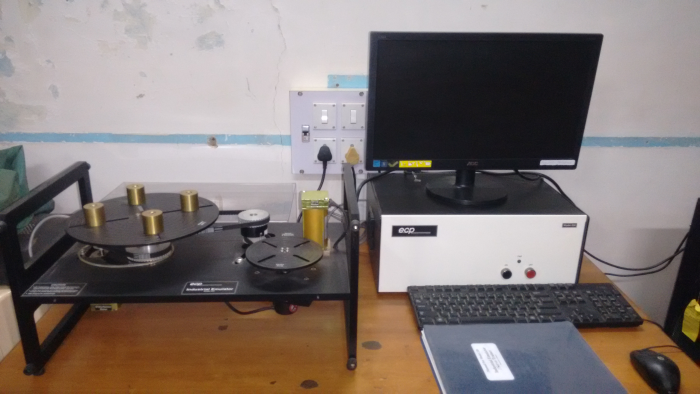
\includegraphics[width = \textwidth]{full.png}
\caption{Industrial Emulator Set-up}
\label{Fig1}
\end{figure}
\subsection{Why called 'Industrial Emulator'?}
The reason why the plant is known as ’Industrial Emulator’ is because it has many configurable features present in real industrial plants which are: \\
\begin{itemize}
\item Rigid bodies
\item Flexibility in drive shaft, gearing and shafts.
\item Coupled discrete vibration with actuator at the drive input and sensor collocated or non-collocated.
\end{itemize}
Also following non-ideal properties can be removed and introduced as per need:
\begin{itemize}
\item Backlash
\item Drive Friction
\item Disturbances
\end{itemize}
\subsection{System Overview}
The system has three subsystems
\subsubsection{Electro-Mechanical Plant}
The electro-mechanical plant(Figure \ref{Fig2}) consists of :
\begin{itemize}
\item The plant consisting of drive and load disk which can be coupled with different gear ratios with stiff or flexible belt. The moment of inertia of source and load can be varied by placing brass weights of different masses on the disks.
\item Actuators - DC brushless motors - There is a drive motor which is coupled with the drive disk. A disturbance motor can be used to introduce viscous friction and disturbances in step, ramp, or sinusoidal form.
\item Sensors - High resolution digital encoder which gives accurate measurement of the angular position of the load and drive disks. Encoder 1 and 2 corresponds to drive and load disks respectively.
\end{itemize}
\begin{figure}[H]
\centering
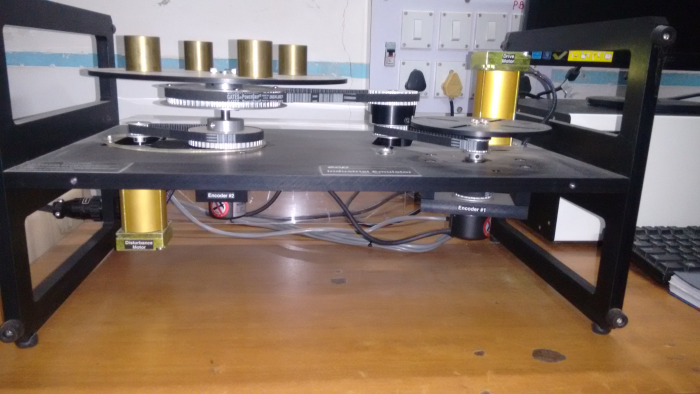
\includegraphics[width = \textwidth]{plant.png}
\caption{Electro-mechanical Plant}
\label{Fig2}
\end{figure}
\subsubsection{Real-time Controller}
It consists of:
\begin{itemize}
\item Digital Signal Processor(DSP) based real-time controller (digital controller)
\item Servo/actuator interfaces - Digital to Analog Converters (DAC) and Analog to Digital Converters(ADC)
\item Servo amplifiers
\item Auxiliary Power Supplies
\end{itemize}
\subsubsection{User Interface Software- ECP Software}
Through the software controller specification, trajectory definition, data acquisition, plotting, system execution commands etc. can be performed. The interface is as shown in figure \ref{Fig3}
\begin{figure}[H]
\centering
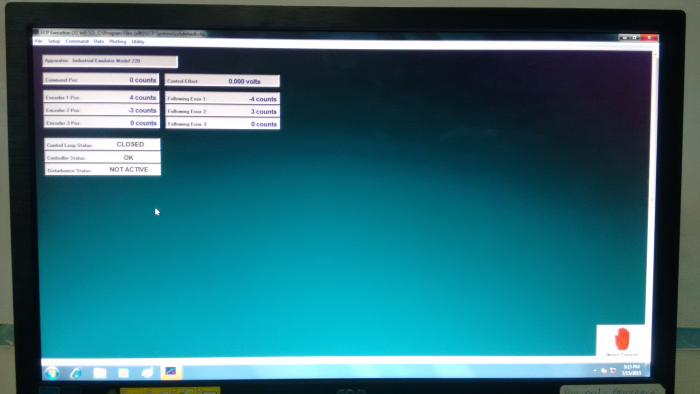
\includegraphics[width = \textwidth]{sw_interface.png}
\caption{ECP Software Interface}
\label{Fig3}
\end{figure}
\begin{figure}[H]
\centering
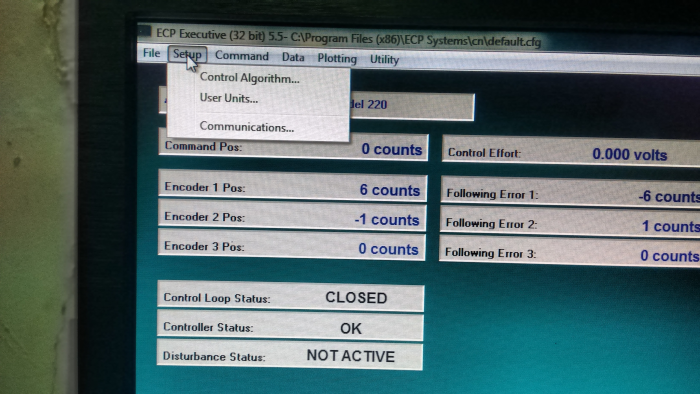
\includegraphics[width = \textwidth]{setup_menu.png}
\caption{Setup Menu}
\label{Fig4}
\end{figure}
\begin{itemize}
\item In the main screen there are encoder positions, commanded position, control effort and status of controller, disturbance and control loop. Abort button is there to immediately open the loop in case of undesirable response.
\item In the ‘file’ menu there is facility to load settings as ‘.cfg’ file. The present settings can be saved as well.
\item In the ‘setup’ menu(figure \ref{Fig4}) the control algorithm can be configured and implemented via ‘setup control algorithm’. Units of measurements can be changed from counts to degrees or radians from ‘user units’.
\item Under the ‘command’ menu the input trajectories and disturbances can be selected and executed.
\item In ‘Data Acquisition’ the instructions on what variables has to be recorded and in how many servo cycles can be given.
\item Under ‘Plot’ different acquired data can be plotted, saved etc.
\item In ‘Utility’ the controller can be reset, encoders can be positioned to zero, motor can be rephased etc.
\end{itemize}
\subsection{Hardware System}
The plant, shown in figure \ref{Fig5} is designed to emulate a broad range of typical servo control applications. The Model 220 apparatus consists of a drive motor (servo actuator) which is coupled via a timing belt to a drive disk with variable inertia. Another timing belt connects the drive disk to the speed reduction (SR) assembly while a third belt completes the drive train to the load disk. The load and drive disks have variable inertia which may be adjusted by moving (or removing) brass weights. Speed reduction is adjusted by interchangeable belt pulleys in the SR assembly. Backlash may be introduced through a mechanism incorporated in the SR assembly, and flexibility may be introduced by an elastic belt1 between the SR assembly and the drive disk. The drive disk moves one-for-one with the drive motor so that its inertia may be thought of as being collocated with the motor. The load inertia however will rotate at a different speed than the drive motor due to the speed reduction. Also, drive flexibility and/or backlash may exist between it and the drive motor and hence its inertia is considered to be noncollocated with the motors.
\begin{figure}[H]
\centering
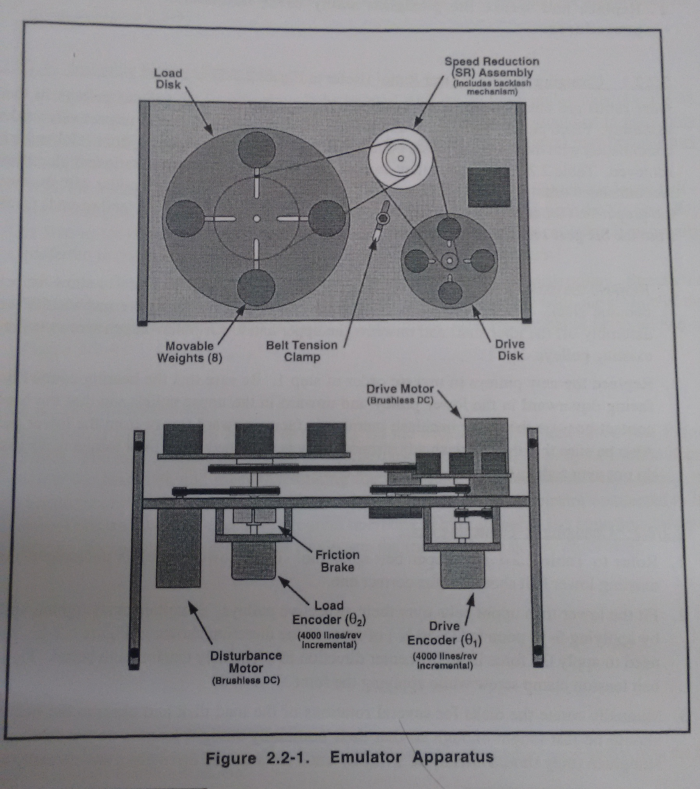
\includegraphics[width = \textwidth]{hw_setup.png}
\caption{Emulator apparatus}
\label{Fig5}
\end{figure}
A disturbance motor connects to the load disk via a 4:1 speed reduction and is used to emulate viscous friction and disturbances at the plant output. A brake below the load disk may be used to introduce Coulomb friction. Thus friction, disturbances, backlash, and flexibility may all be introduced in a controlled manner. These effects represent non-ideal conditions that are present to some degree in virtually all physically realizable electromechanical systems. \\ \\
All rotating shafts of the mechanism are supported by precision ball bearings. Needle bearings in the SR assembly provide low friction backlash motion (when backlash is desired). \\ \\
High resolution incremental encoders couple directly to the drive ($\theta_1$) and load ($\theta_2$) disks providing position (and derived rate) feedback. The drive and disturbance motors are electrically driven by servo amplifiers and power supplies in the Controller Box. The encoders are routed through the Controller box to interface directly with the DSP board via a gate array that converts their pulse signals to numerical values.
\subsubsection{Changing Configuration}
\textbf{Changing Pulleys and Gear Ratio:} Gear ratios are changed via selection of the sizes of the upper and lower pulleys in the SR assembly. Fixed pulleys at the drive and inertia disks have 12 and 72 teeth respectively so that in combination with the interchangeable pulleys, end-to-end gear ratios ranging from 1.5:1 to 24:1 are achieved.
\begin{enumerate}
\item Loosen the ‘Belt Tension Clamp’ (figure \ref{Fig5}).
\item Remove belts.
\item Loosen the backlash screw and then the clamp screw. (figure \ref{Fig7})
\item Remove upper and lower parts and unscrew the bottom and upper pulleys.
\item Repeat the above steps in \textbf{reverse order} with new pulleys. Make sure the belts are selected properly.(figure \ref{Fig6}). Also make sure both the belts are taught.If they are slack they may add flexibility which is unwanted.
\end{enumerate}
\begin{figure}[H]
\centering
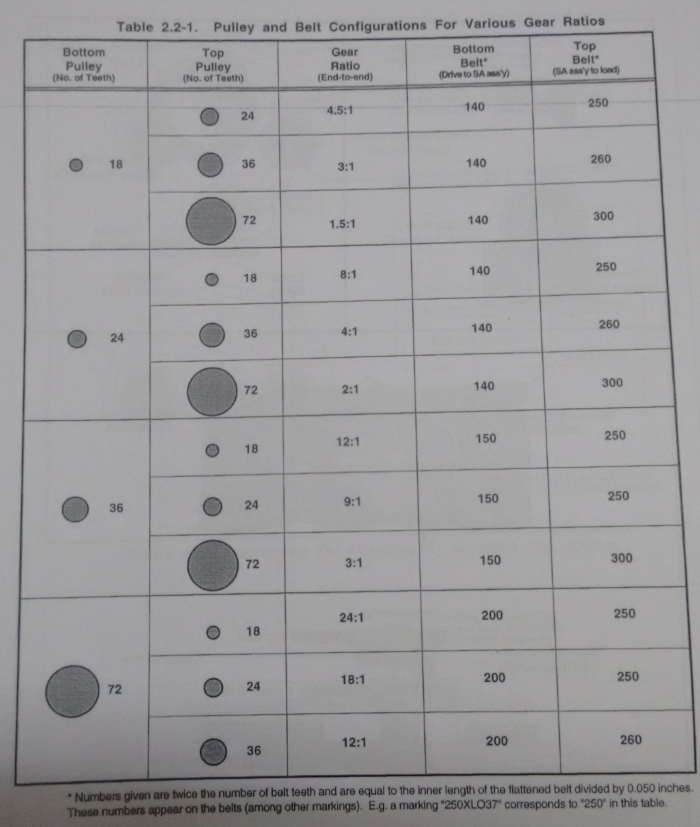
\includegraphics[width = \textwidth]{pulley_config.png}
\caption{Pulley and Belt Configurations for Various Gear Ratios}
\label{Fig6}
\end{figure}
\begin{figure}[H]
\centering
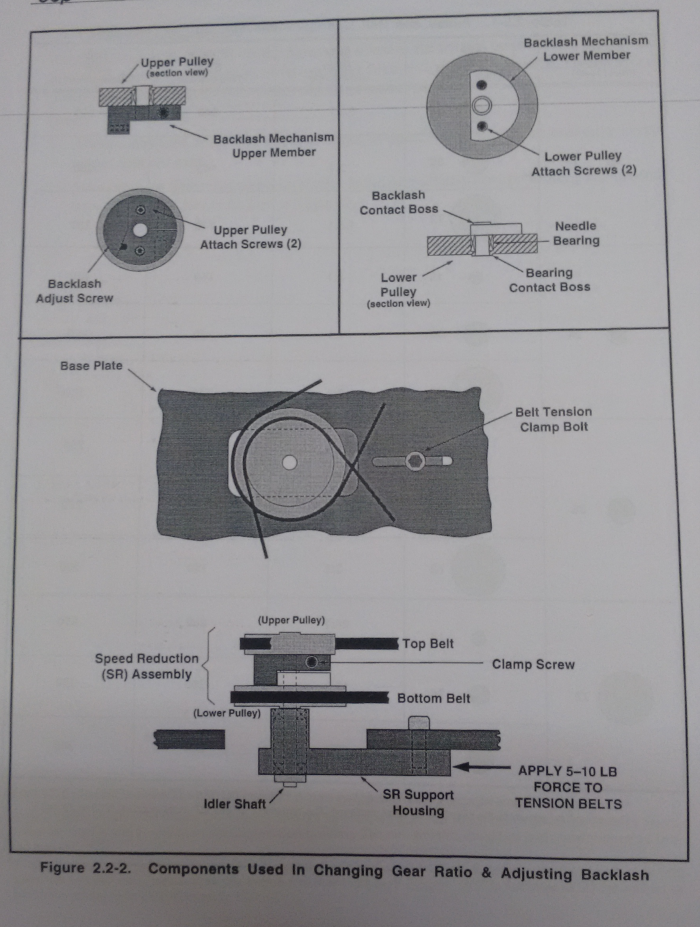
\includegraphics[width = \textwidth]{gr_backlash.png}
\caption{Components used in changing Gear Ratio and Changing Backlash}
\label{Fig7}
\end{figure}
\textbf{Changing Brass Weights:} Unscrew the weights from the disk and place new ones on the concentric circle lining according to where it has to be placed. The first circle is of radius 2cm and the outer ones are increased at 1cm. \\ \\ 
\textbf{Installing Flexible Belts:} It is recommended that the flexible drive belts be used with the 36 tooth pulley only (I.e. the 36 tooth pulley in the upper position in the SR assembly.) \textbf{The flexible belt should be in place only for the duration of active testing.} Prolonged periods (more than several hours) may permanently stretch the belts.
\begin{enumerate}
\item With upper belt removed, tighten the lower belt. It is usually preferred to position the SR assembly as close as possible to the load disk.
\item Now stretch the flexible belt and place fit it around the upper pulley.
\end{enumerate}
\textbf{Adjusting Backlash} Backlash is adjusted (0 to 20 deg @ the SR) via the backlash adjustment screw (see figure \ref{Fig7}). The amount of backlash is measured by temporarily tightening the friction clamp below the load disk(i.e., make load disk immovable and rotate the drive disk) and manually rotating the drive disk back and forth while noting the encoder readings at each extreme. \textbf{Be certain that you loosen the friction clamp before proceeding.} \\ \\ 
\textbf{Adjusting Friction Brake} Coulomb friction is adjusted via the tightening screw in the friction brake. The brake should not be set greater than 1 N-m to avoid excessive friction and hence excessive drive current (under subsequent closed loop control) which can lead to amplifier burn-out. \textbf{Always loosen the brake after performing any necessary tests.}
\subsection{Do's and Dont's}
\begin{itemize}
\item While turning ON, first start the PC, then turn on the control box. While turning OFF, first turn OFF the control box and then turn off the system.
\item Use Abort control if any undesirable response occurs during tests.
\item Stay clear of and do not touch any part of the mechanism while it is moving, while a trajectory has been commanded (via Execute, Command menu), or before the active controller has been safety
\item Do not take the cover off or physically touch the interior of the Control Box unless its power cord is unplugged (first press the ”Off” button on the front panel) and the PC is unpowered or disconnected.
\item Stay clear of the mechanism while wearing loose clothing (e.g. ties, scarves and loose sleeves) and when hair is not kept close to the head.
\item Keep head and face well clear of the mechanism.
\end{itemize}
\section{Experiment - Fundamentals of Servo Control}
In this section we consider the effects of changes in parameters and of certain properties that are present in most control systems and in all digitally controlled mechanical systems. These effects have implications to design and analysis of the mechanism, control hardware and control scheme. While the work in this section shall include only PD, PID and simple filter control, the effects studied have implications to all practical control methodologies. \\
In some cases we shall control the system about the drive disk and in some about the load disk. The former is referred to as collocated control since the sensor and actuator are rigidly coupled and hence kinematically lie at the same location. The latter potentially involves flexibility, backlash, and drive nonlinearity between the actuator and sensor and is referred to as noncollocated control.\\
We use the test cases from figure \ref{Fig8} to perform the experiments.
\begin{figure}[H]
\centering
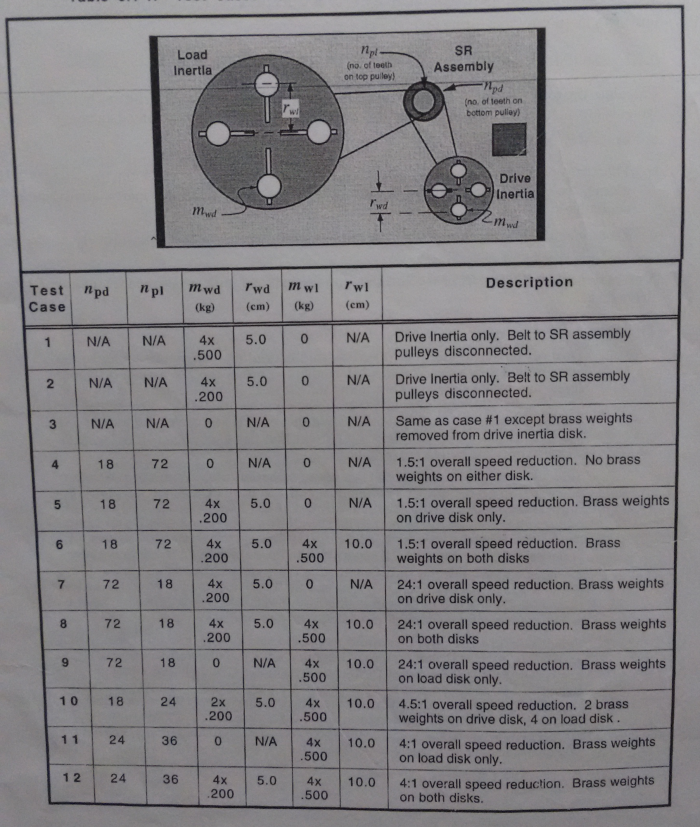
\includegraphics[width = \textwidth]{test_cases.png}
\caption{Test Cases}
\label{Fig8}
\end{figure}
\subsection{Effect of Gear Ratio and Inertia}
Gear ratio and inertia have fundamental effects on the system dynamics since they effectively scale the system gain. In the procedure that follows these relationships are demonstrated experimentally.
\begin{enumerate}
\item Set-up the system in the configuration of Test Case 6.(figure \ref{Fig8})
\item Setup to collect data every 1 servo cycle. Utilizing the underdamped PD controller in experiment 2 with $Ts = 0.00884 s$, execute a 2000 count Step of 2500 ms duration. Compare the response with that from the Experiment 2 underdamped case. Save your plot. Measure the damped natural frequency $\omega_d$, calculate $\omega_n$ and $\eta$ for both cases. Now change the gear ratio to 24:1 and repeat the above procedure and calculations for Test Cases 8 and 9.
\end{enumerate}
\subsubsection{Plots}
\begin{figure}[H]
\centering
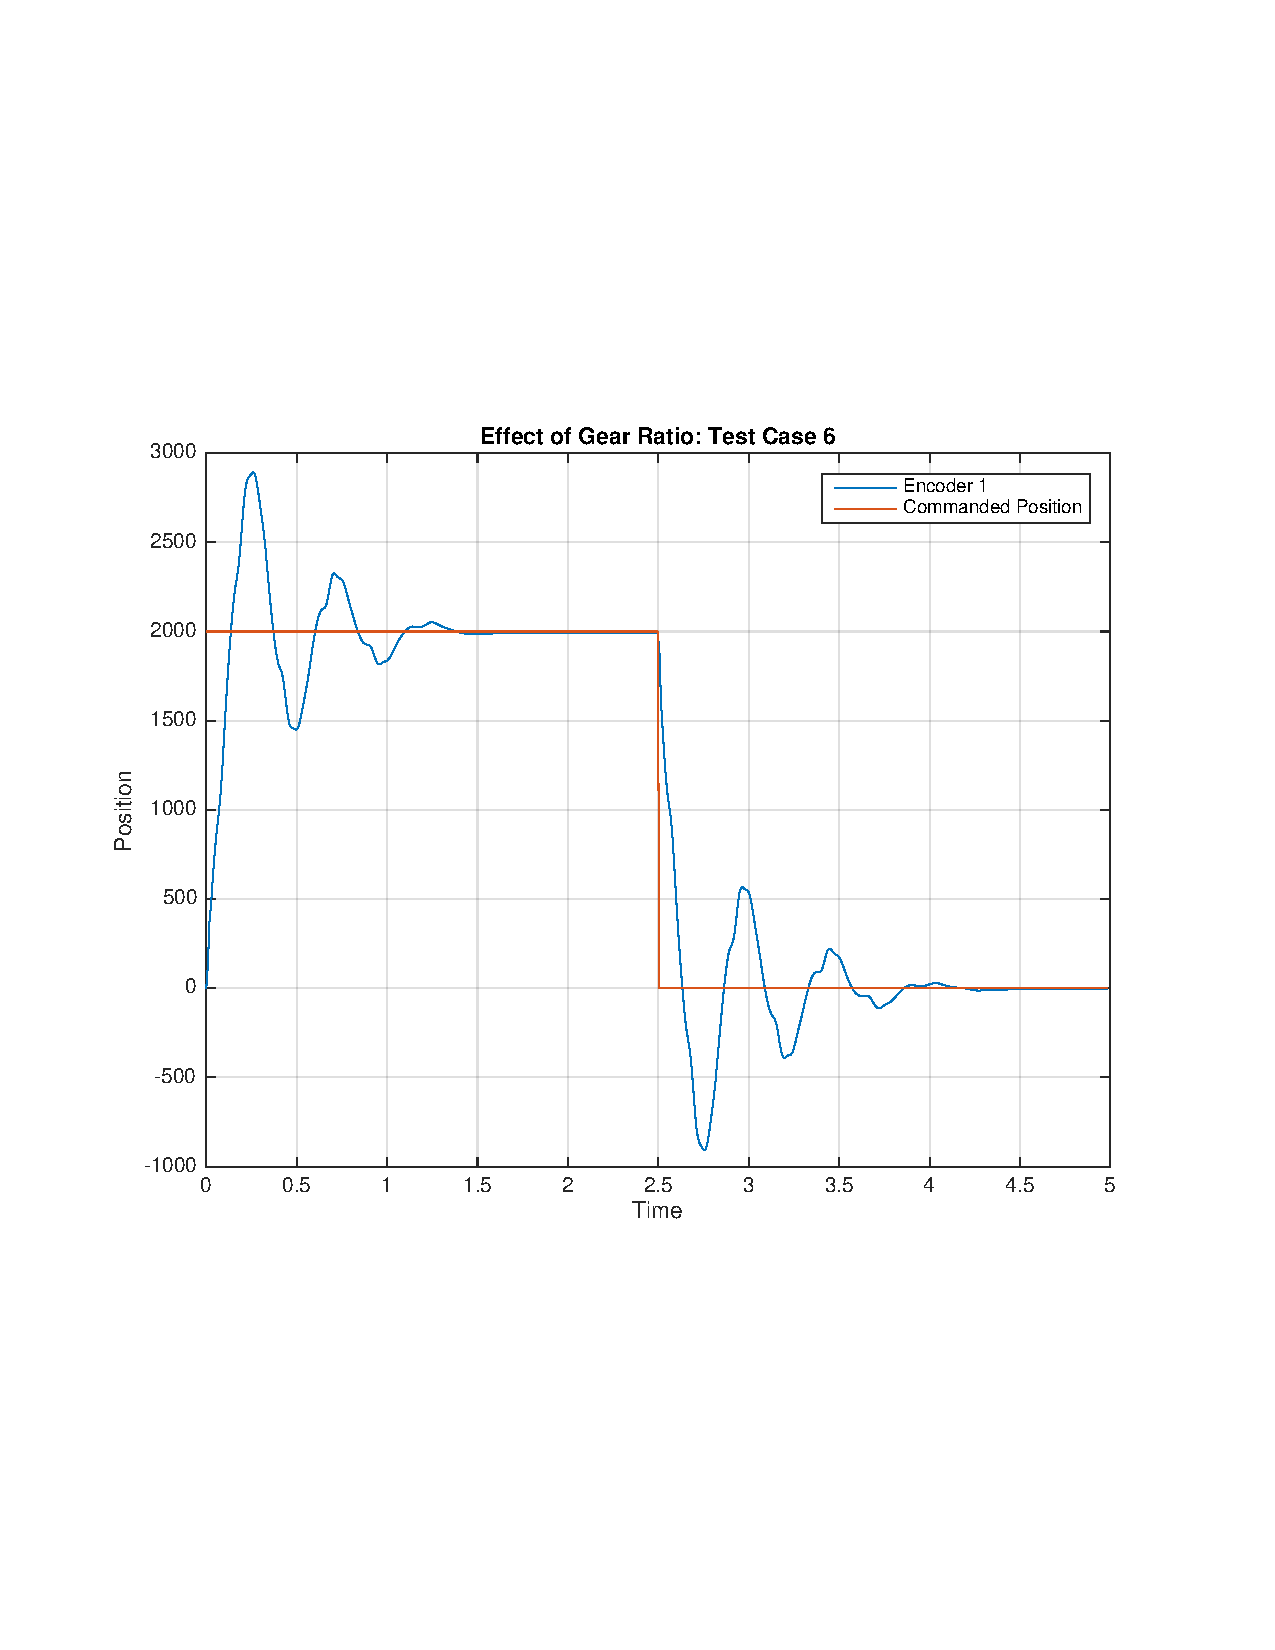
\includegraphics[width = \textwidth]{gr_tc6.pdf}
\caption{Underdamped PD response with Gear Ratio 1.5}
\end{figure}
\begin{figure}[H]
\centering
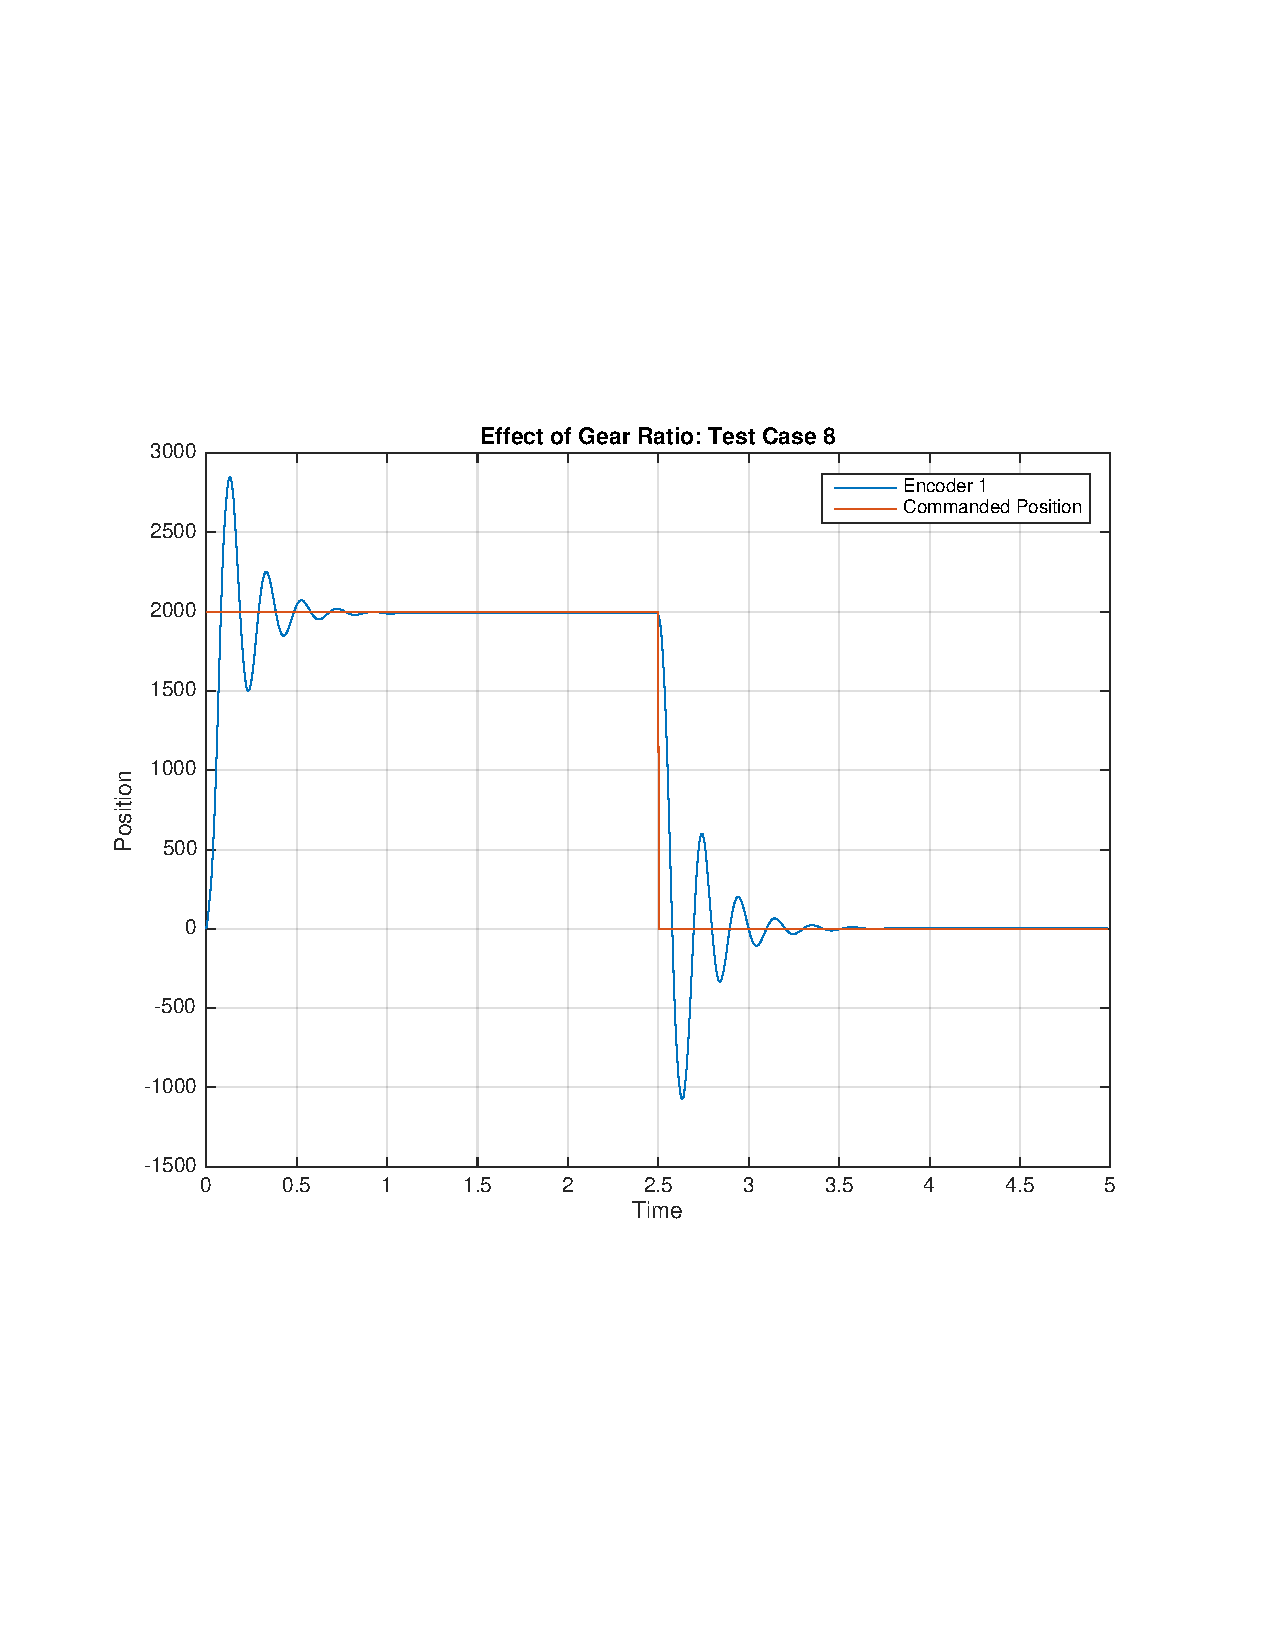
\includegraphics[width = \textwidth]{gr_tc8.pdf}
\caption{Underdamped PD response with Gear Ratio 24 with test case 8}
\end{figure}
\begin{figure}[H]
\centering
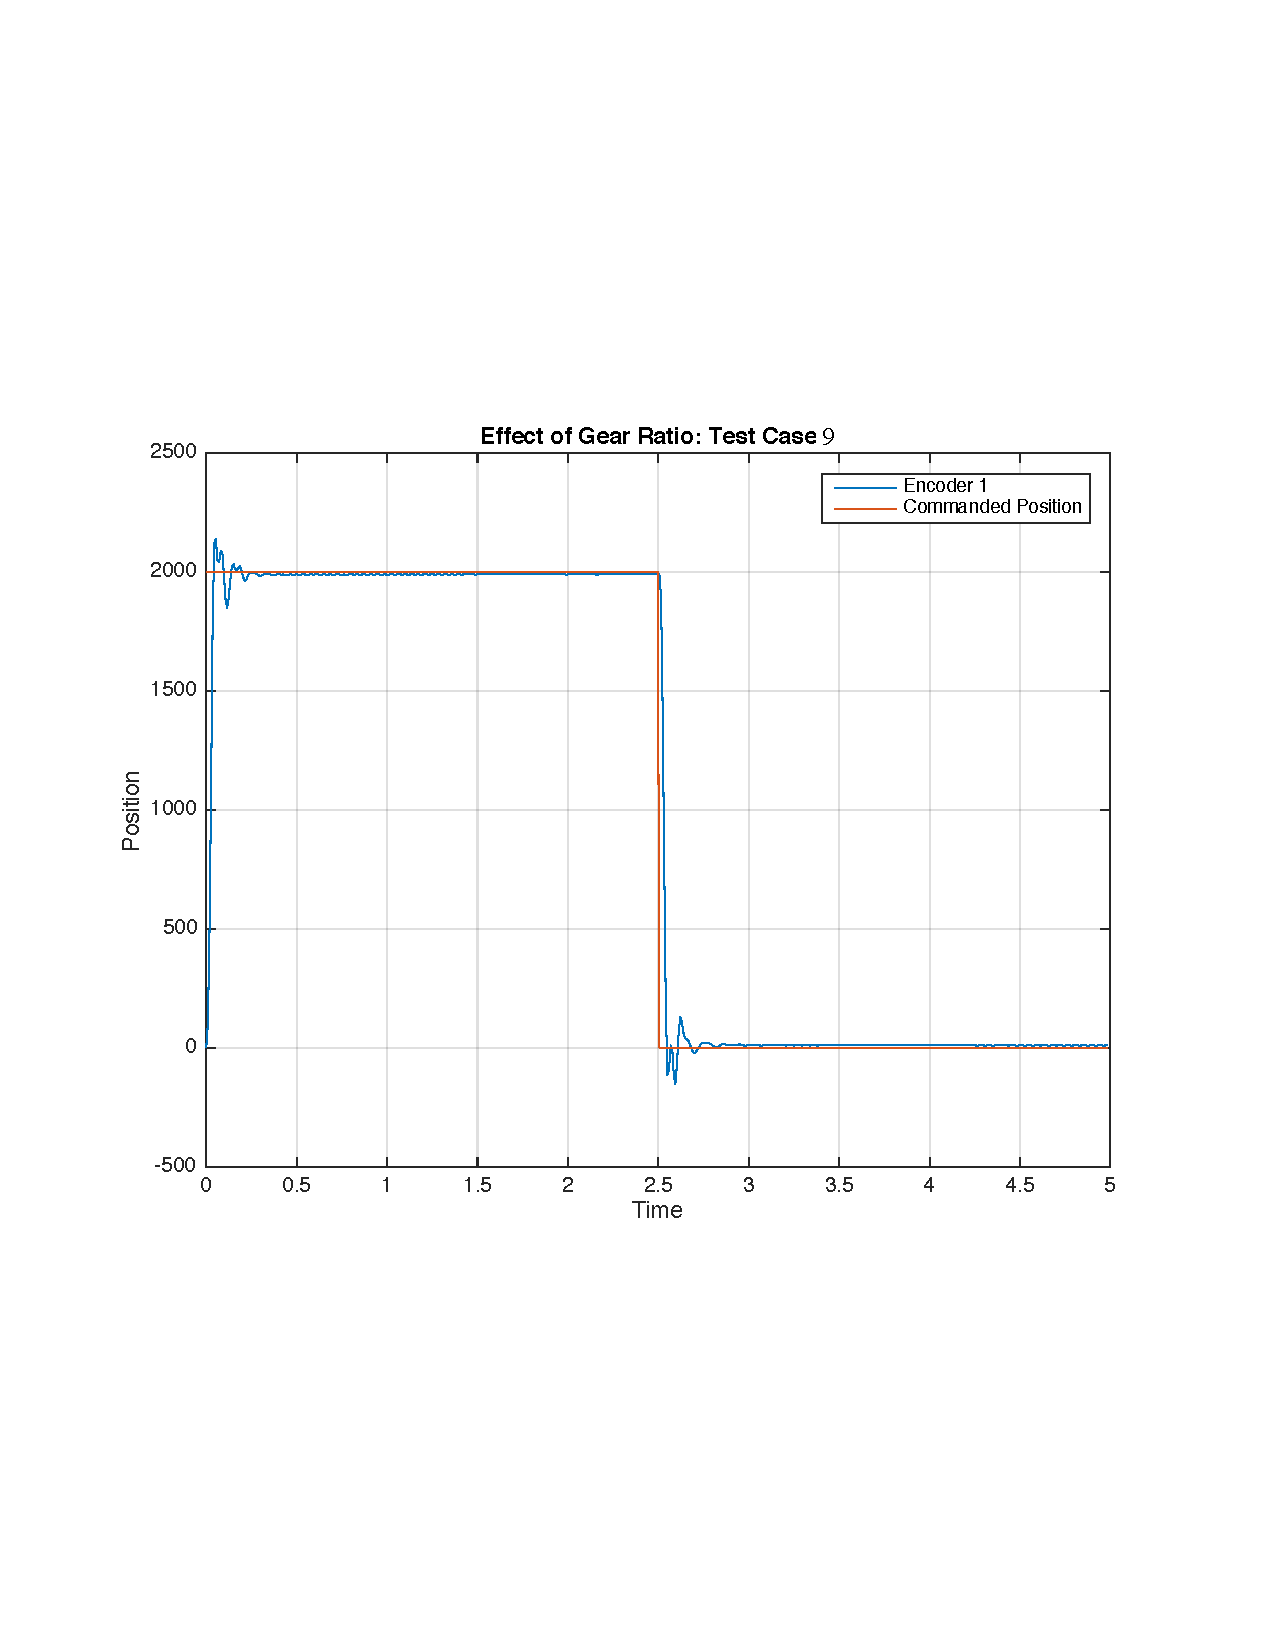
\includegraphics[width = \textwidth]{gr_tc9.pdf}
\caption{Underdamped PD response with Gear Ratio 24 with test case 9}
\end{figure}
\subsection{Effect of Friction}
Friction exists to some extent in all practical mechanical systems. It may be modeled as being a combination of static and Coulomb (kinetic) and viscous types. Coulomb and static(figure \ref{Fig12}) friction are often of greater magnitude than viscous and exacerbate the control design problem in that they are nonlinear. In small amounts they may actually help to stabilize a system, but are generally deleterious to tracking and regulation performance. In this section we consider the effect of Coulomb and static friction at the load output and the dependence of performance on gear ratio and sensor location.
\begin{figure}[H]
\centering
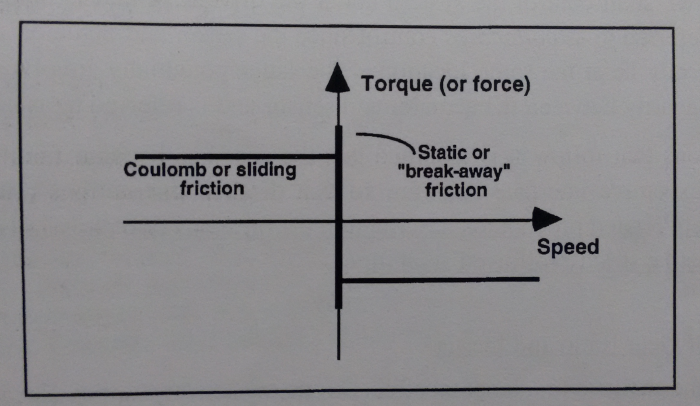
\includegraphics[width = \textwidth]{coulomb_friction.png}
\caption{Simplified model of static and coulomb friction}
\label{Fig12}
\end{figure}
\begin{enumerate}
\item Assure that power to the Controller Box is turned off. Turn the apparatus on its side so that the inertia disks are vertical and the underside is accessible. Tighten the friction brake clamp so that approximately 0.5 N-m of friction torque is applied to the load shaft when it rotates. This may be achieved by placing a single 500 g brass weight at r=10 cm on the load disk. With the weight roughly horizontal relative to the load shaft, adjust the clamp such that the load disk rotates very slowly (or rotation is initiated by very slight downward force on the weight). I.e. the friction torque is approximately equal to the torque generated by gravity acting on the weight. \textbf{Do not over tighten the friction adjustment screw. Only light torque is needed to achieve the desired friction. Over-tightening can damage the clamp and lead to stalling of the motor and potential amplifier burnout.}
\item Configure the mechanism according to Test Case 5(fig. \ref{Fig8}). Power up the Controller Box. Input the following PD gains in the PI with Velocity Feedback dialog box: $k_p = 0.16,k_d = 0.025$. Choose Encoder 1 for feedback and implement the control. Make certain that the encoder positions are nearly zero (within say 10 counts use Zero Position in the Utility menu if necessary). Perform a ramp maneuver with 3000 count distance, 7500 $\frac{count}{s}$ velocity, and 2500 ms dwell. Plot and save the Encoder 2 (load) position response.
\item Determine the gain correction necessary to keep the same nominal closed loop control performance when using the load output sensor (Encoder 2) as the feedback sensor. Correct $k_p$ and $k_d$ accordingly and input these gains under PI with Velocity Feedback choosing Encoder 2 for feedback. Implement the controller and perform a ramp with 2000 count distance, 5000 count/s velocity, and 2500 ms dwell. (nominally the same motion as in Step 2) and again plot the Encoder 2 output. Compare the output with that of Step 2.
\item Repeat Step 2 for the plant in the Test Case 7 configuration using the gains: $k_p = 0.068,k_d = 0.011.$ Repeat step 3.
\end{enumerate}
\subsubsection{Plots}
\begin{figure}[H]
\centering
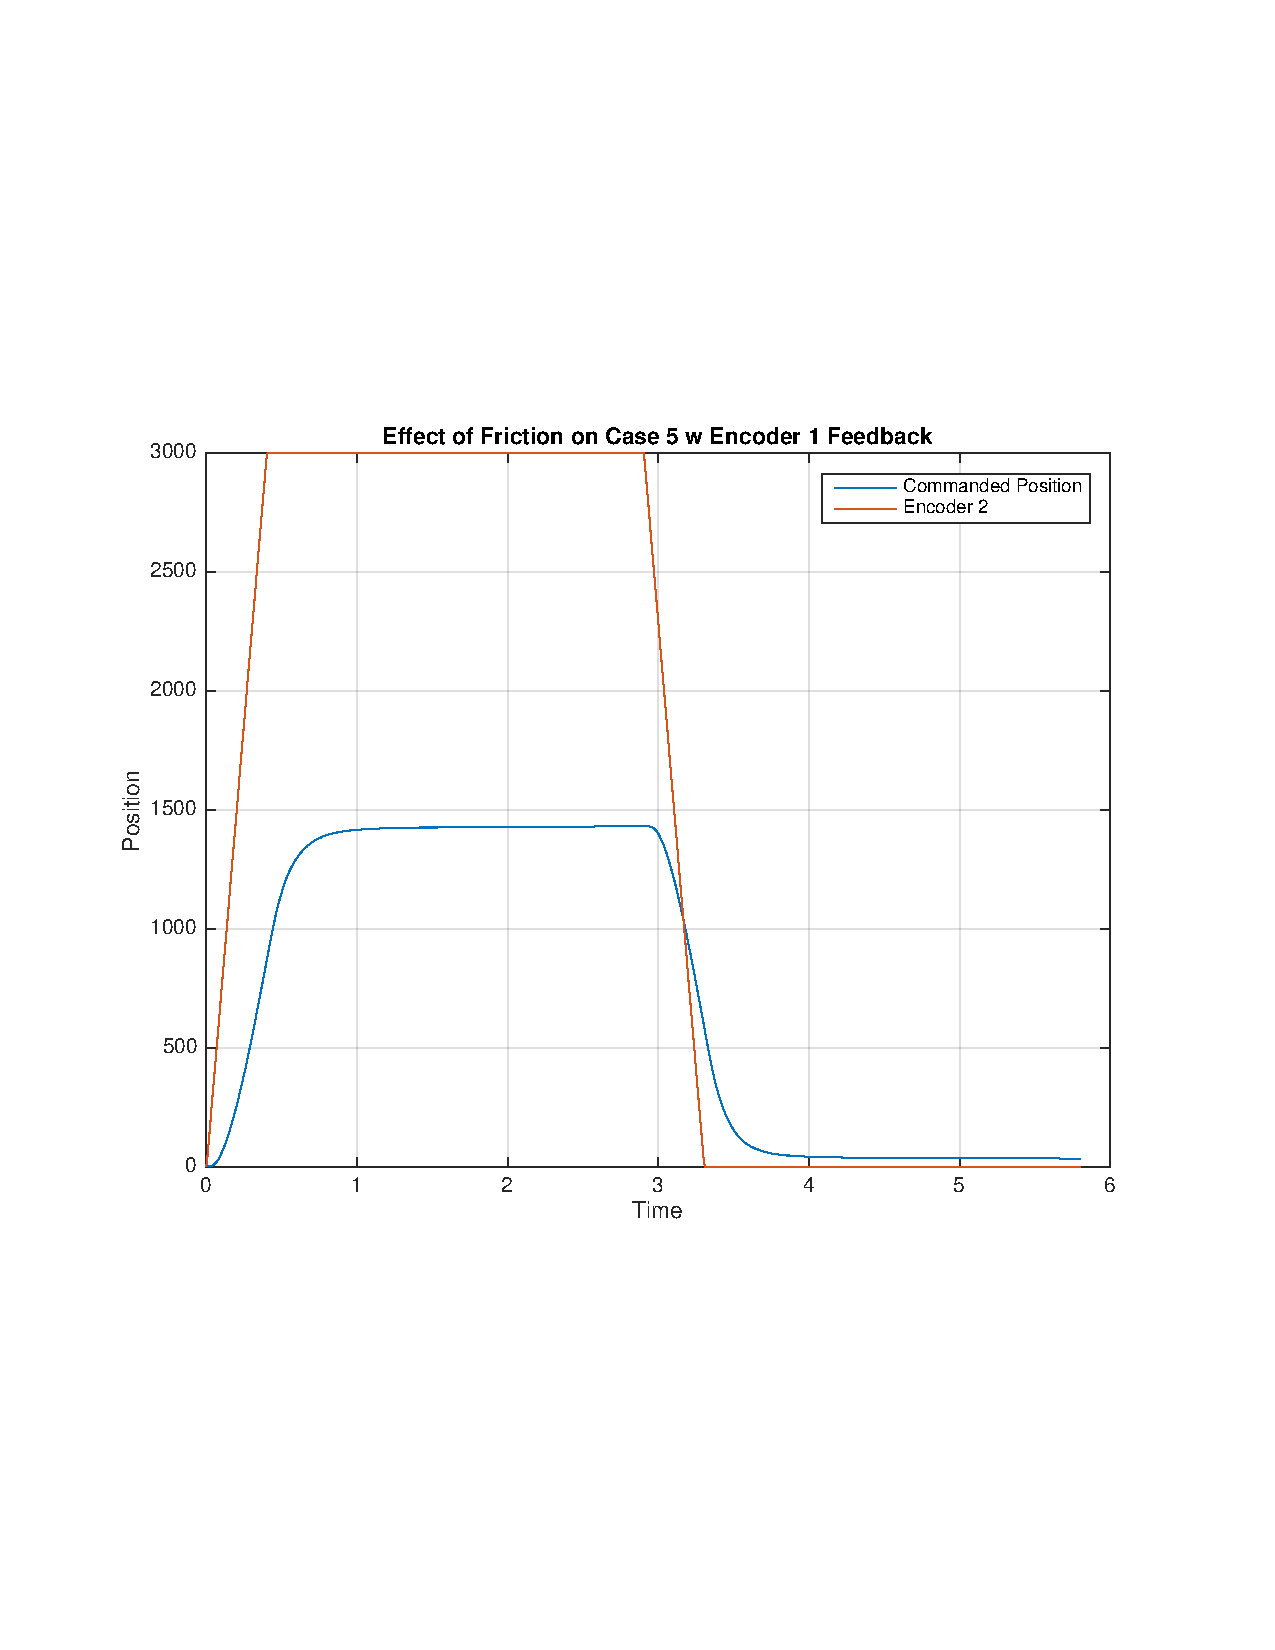
\includegraphics[width = \textwidth]{4_fric.pdf}
\end{figure}
\begin{figure}[H]
\centering
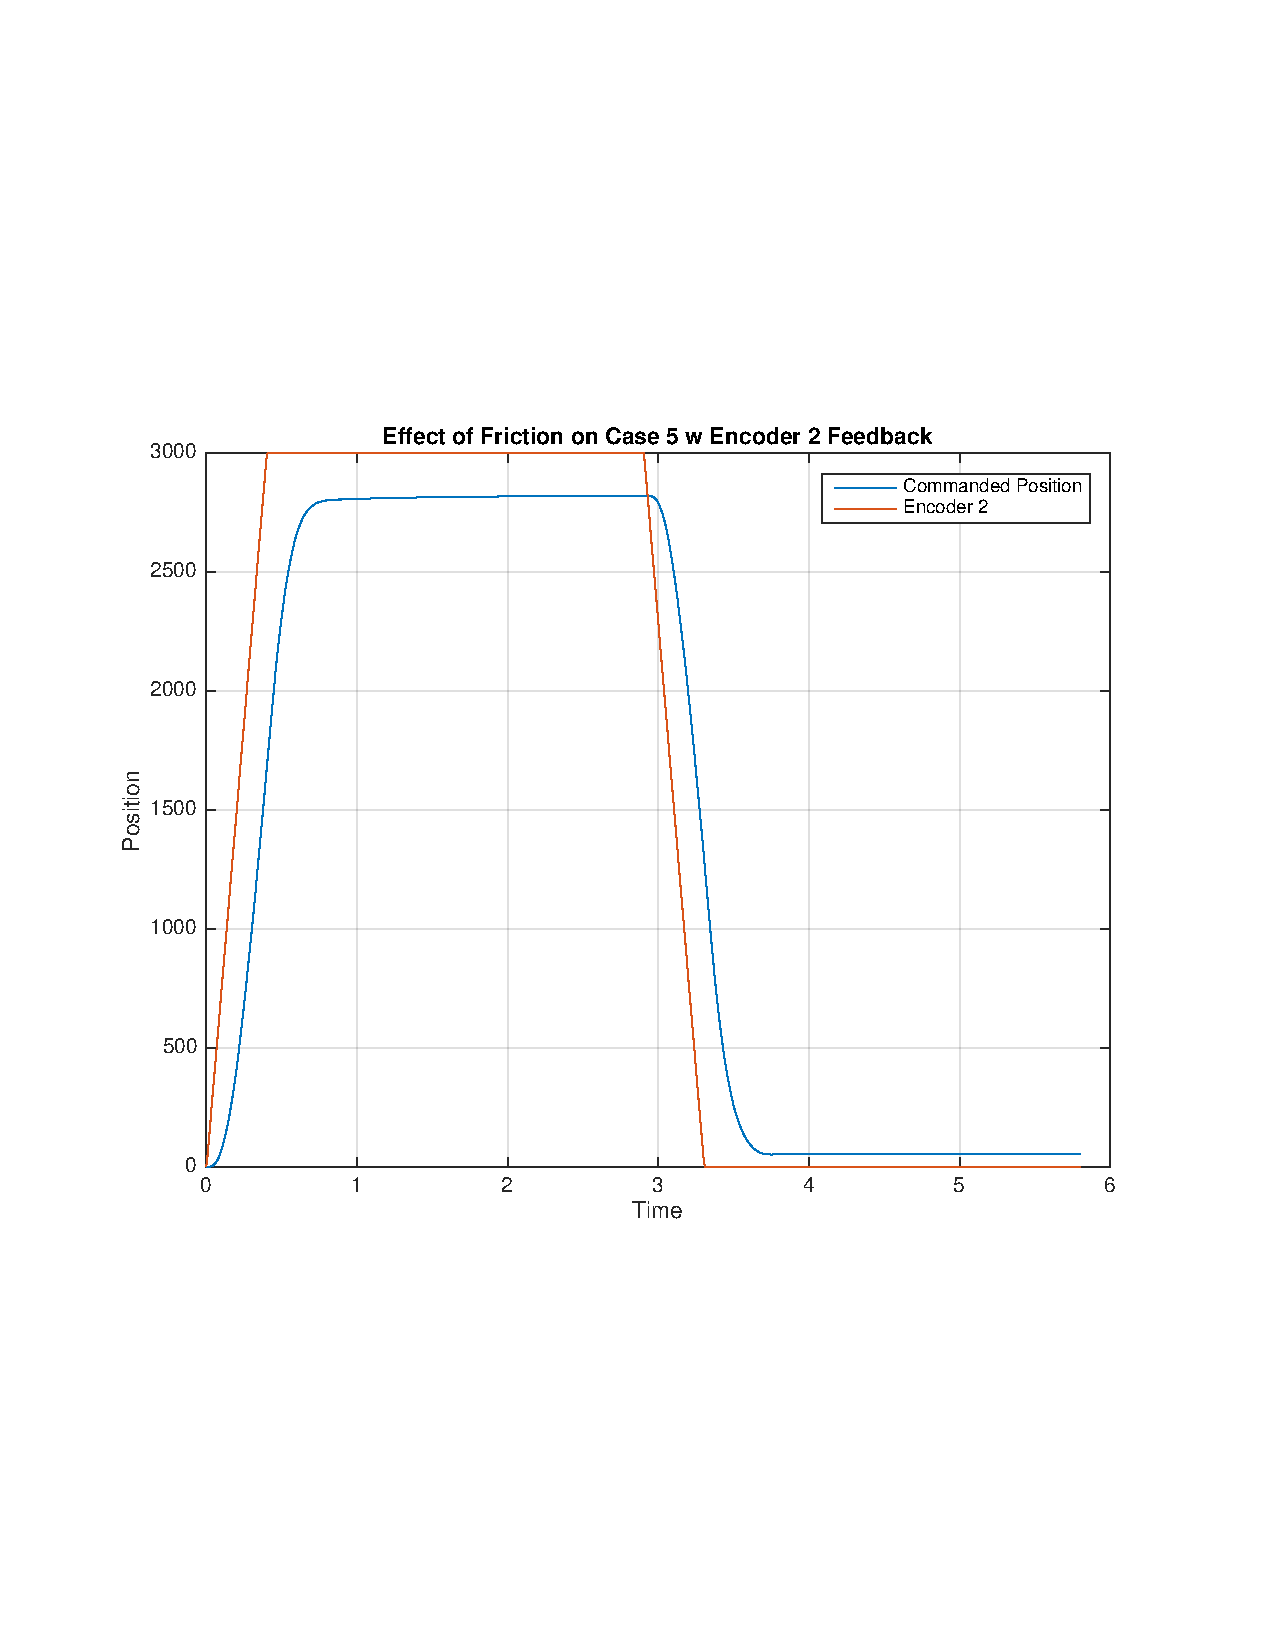
\includegraphics[width = \textwidth]{5_fric.pdf}
\end{figure}
\begin{figure}[H]
\centering
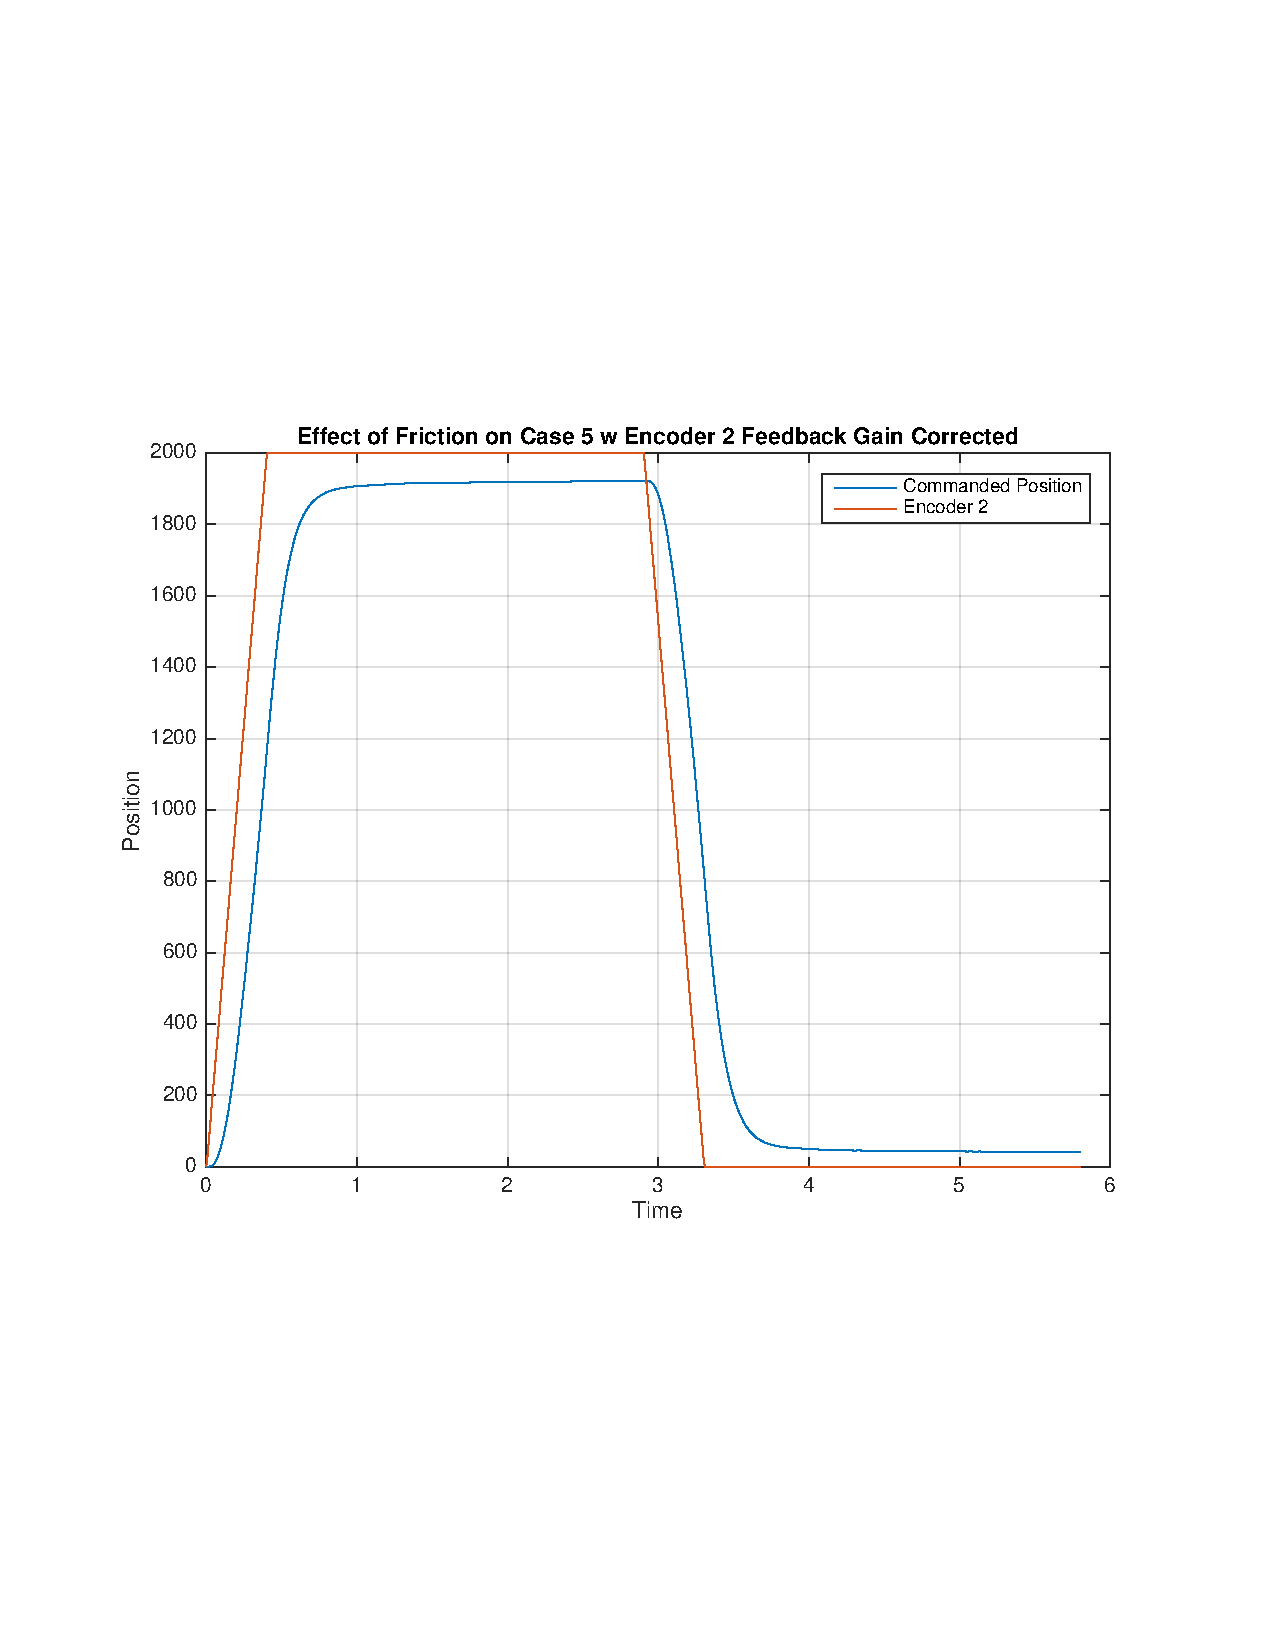
\includegraphics[width = \textwidth]{6_fric.pdf}
\end{figure}
\begin{figure}[H]
\centering
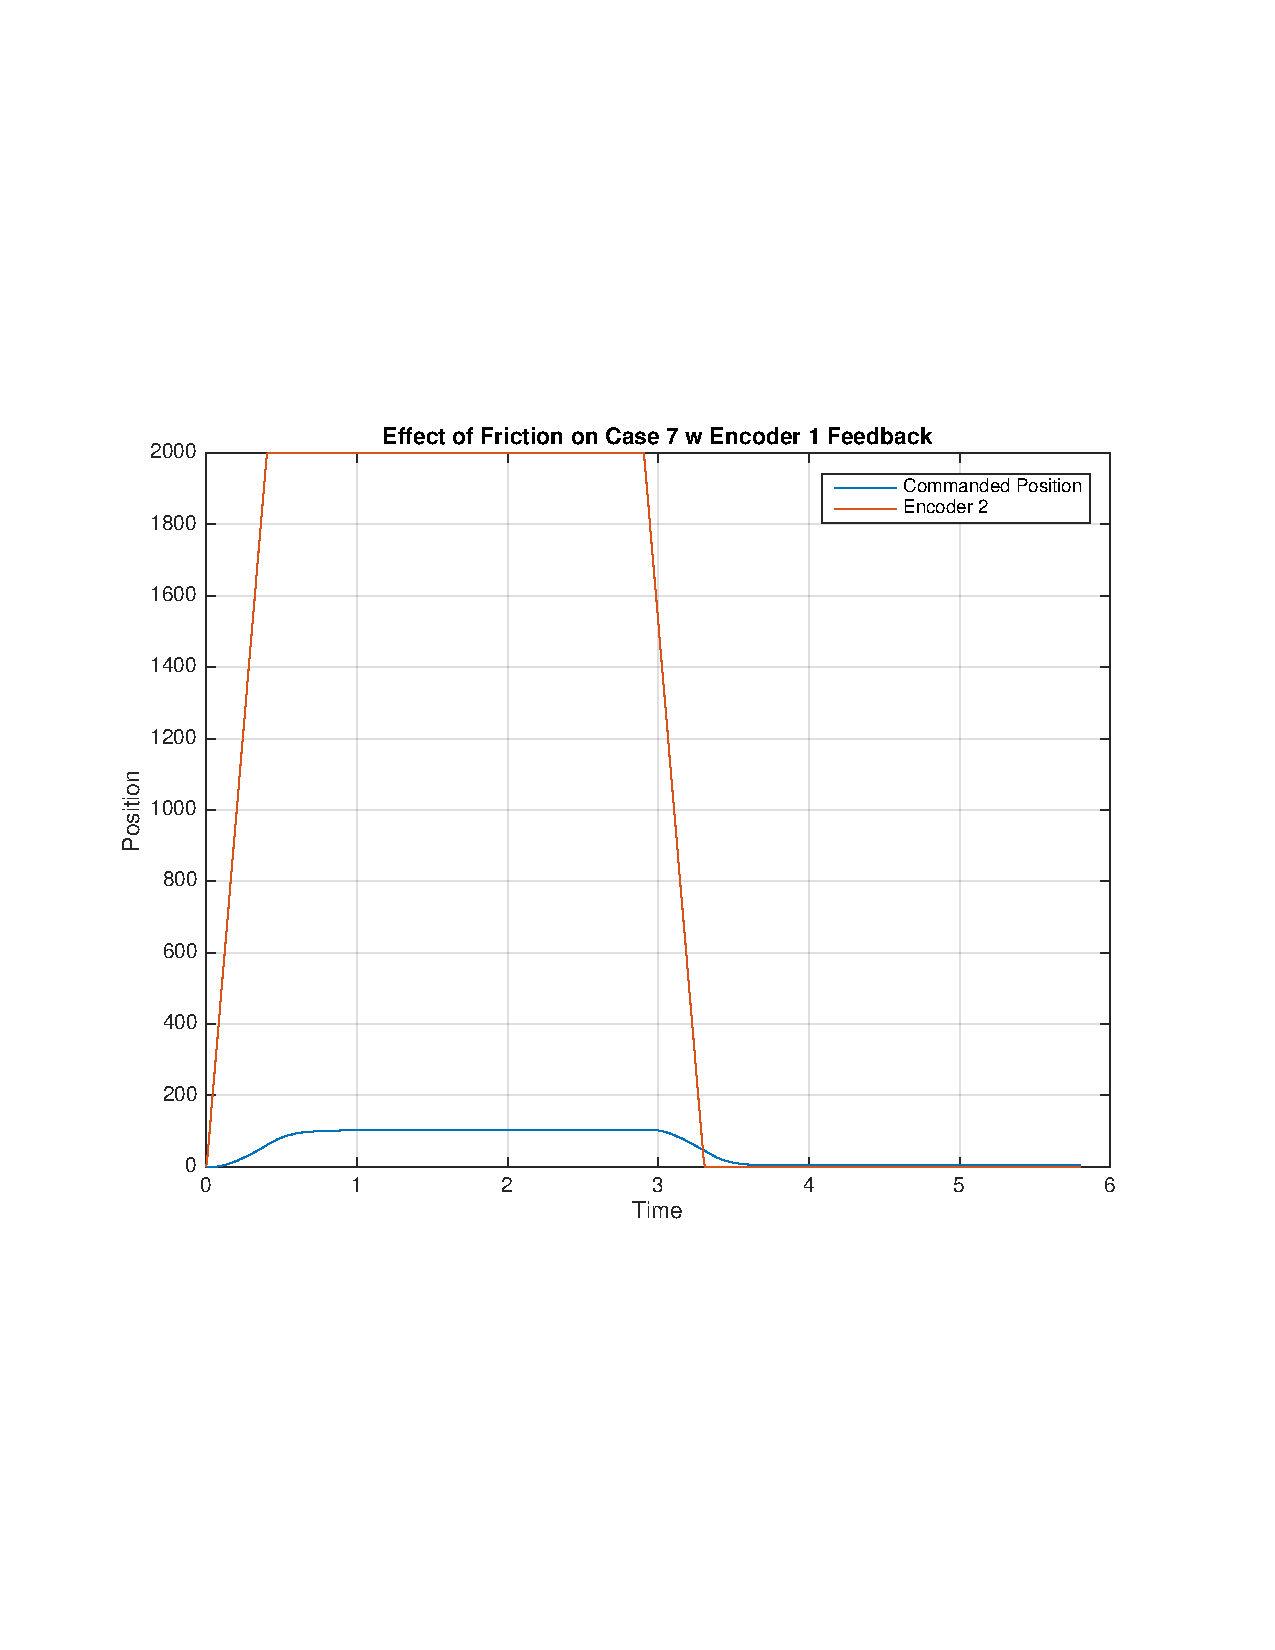
\includegraphics[width = \textwidth]{7_tc7_fric.pdf}
\end{figure}
\begin{figure}[H]
\centering
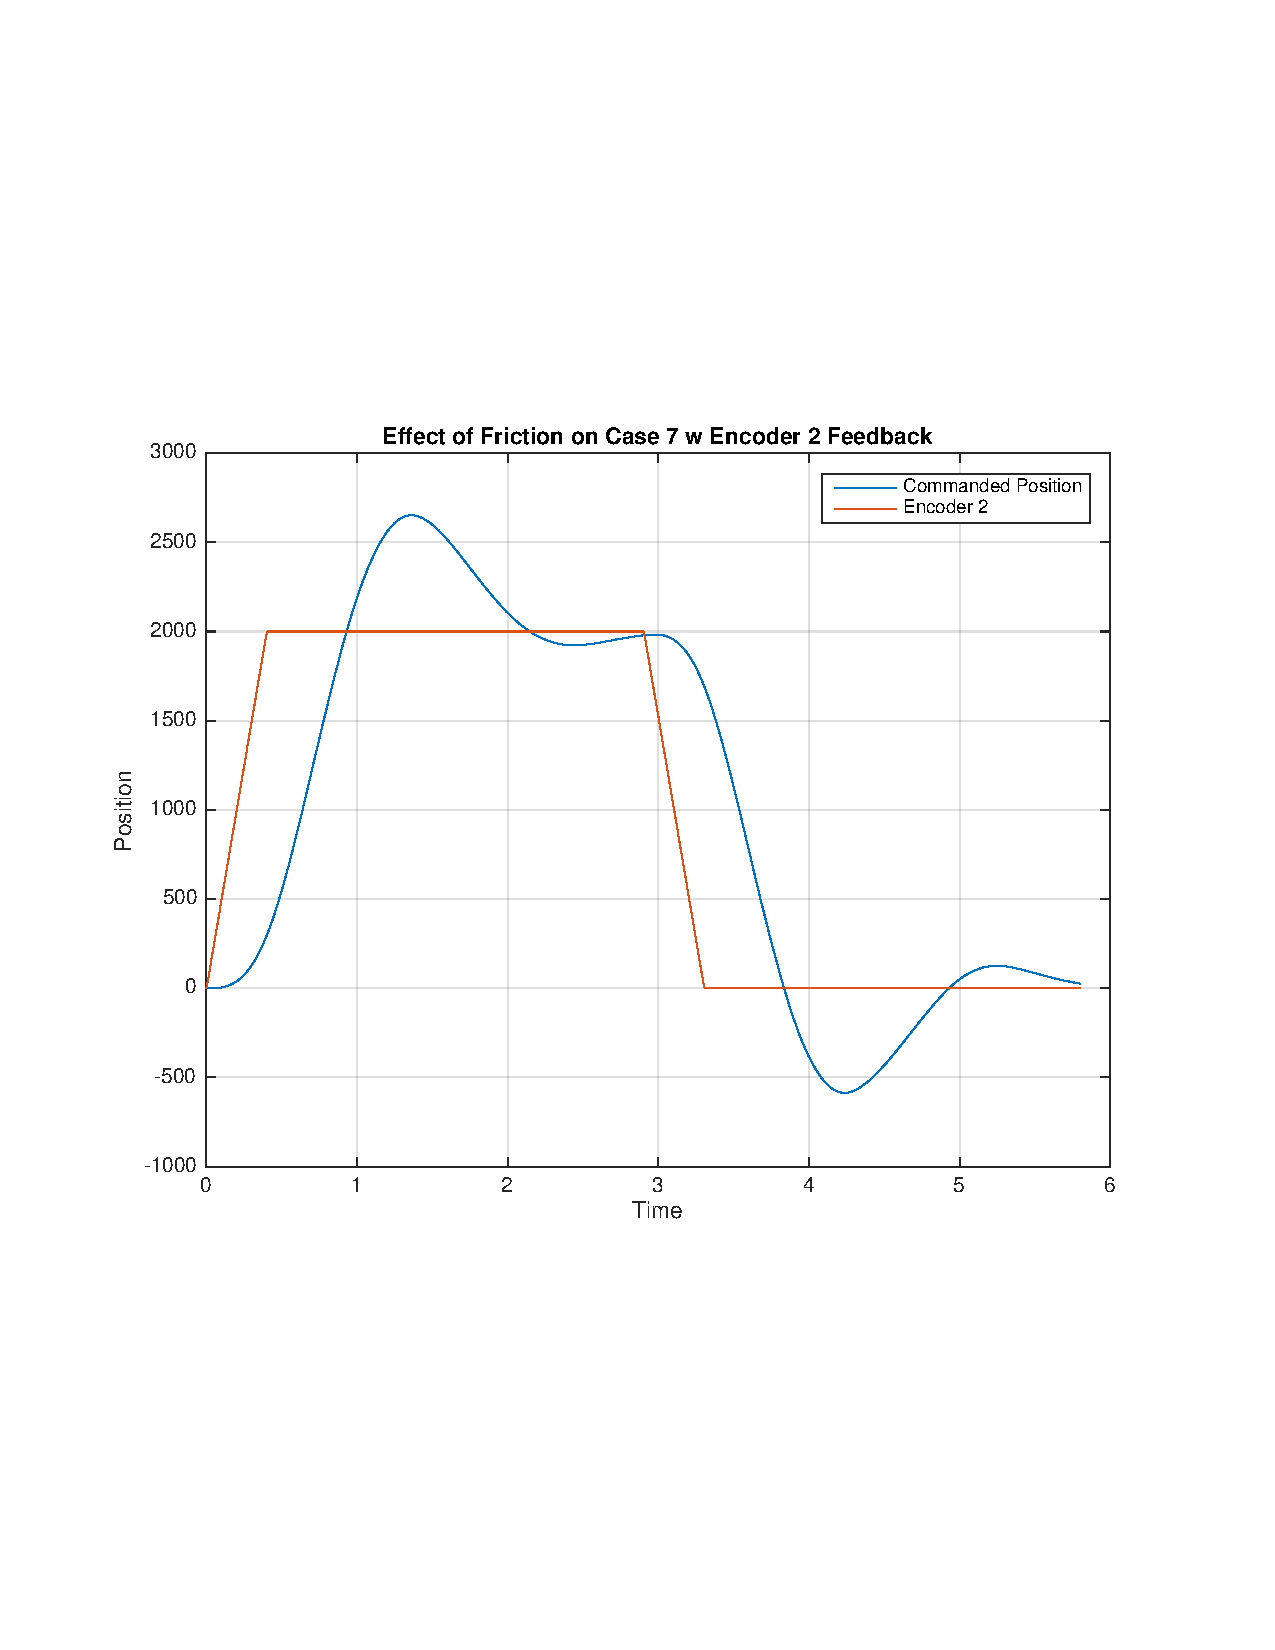
\includegraphics[width = \textwidth]{8_tc7_fric.pdf}
\end{figure}
\begin{figure}[H]
\centering
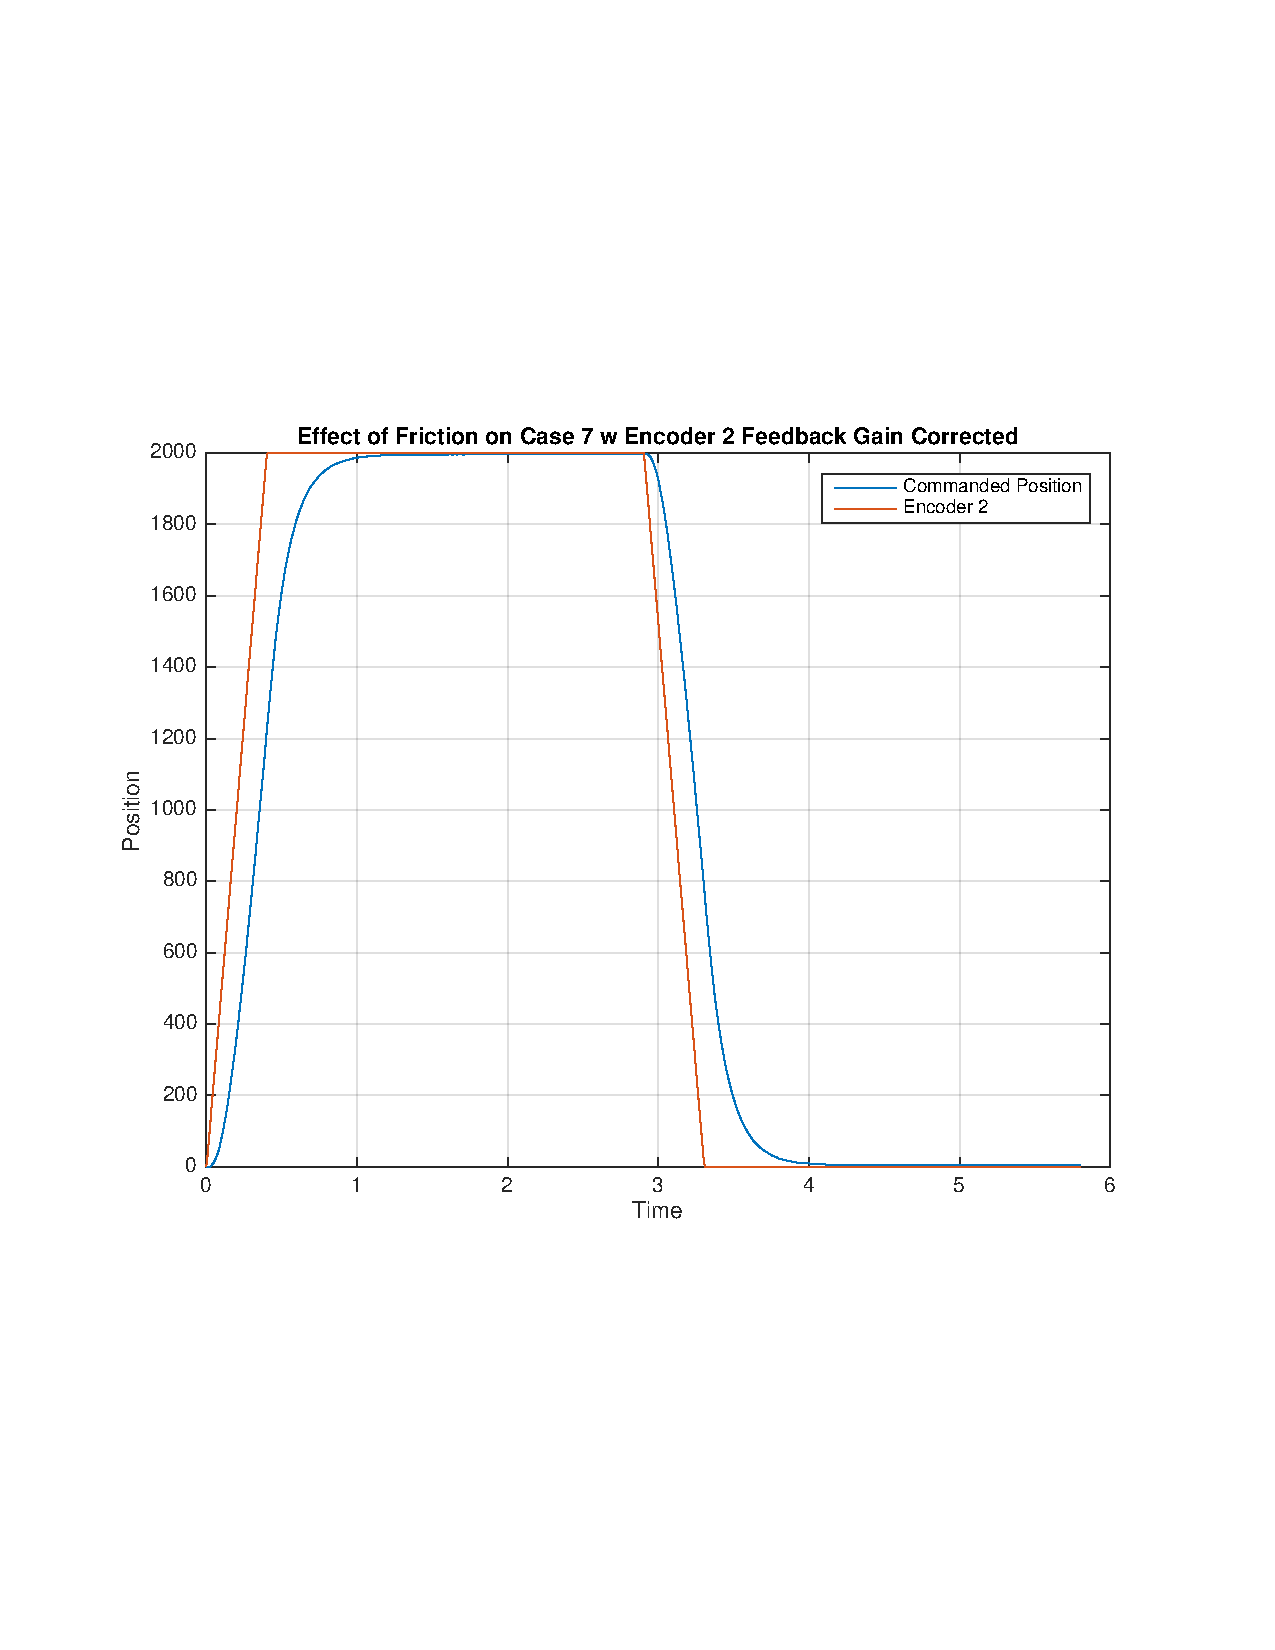
\includegraphics[width = \textwidth]{9_tc7_fric.pdf}
\end{figure}
\subsection{Effect of Disturbances}
In most servo applications, an important requirement of the control design is that it reject forces or torques that tend to disturb the system from its intended set point or tracking trajectory. Examples of disturbances include motor cogging torque, gravity induced loads on the kinematic linkage, interactions with the payload inertia (e.g. material added or removed from a conveyor) and interaction with other operating equipment or control axes (e.g. tool drag on a lathe spindle). In this section we shall consider the effect of slow spatially dependent disturbances as well as low and high frequency time dependent ones. While these effects are studied in the context of tracking and regulation separately, the tracking results are extendible to regulation and vice versa.\\
\textbf{Slow disturbances during tracking (Effect of gear ratio)}
\begin{enumerate}
\item Set up a spatially dependent sinusoidal disturbance (Sinusoidal (theta), under Disturbance, Command menu) of 1.0 volt, 8 cycles/rev., 10,000 ms duration. Input the $k_p$ and $k_d$ values from Step 3 of previous section for the Test Case 5 configuration using PID (not PI with Velocity Feedback) control and Encoder 2 for feedback. With the mechanism set as per Test Case 5, perform a 8000 count ramp maneuver at 2000 counts/s velocity with dwell time of 1000 ms. Make sure that you check the box labeled ”Include sinusoidal disturbance” when commanding the system to execute the trajectory. Plot and save the Commanded Position and Encoder 2 data.
\item Repeat Step 1 for Test Case 7 using $k_p$ and $k_d$ values from Step 4 of previous section under load sensor feedback (Encoder 2).
\end{enumerate}
\subsubsection{Plots}
\begin{figure}[H]
\centering
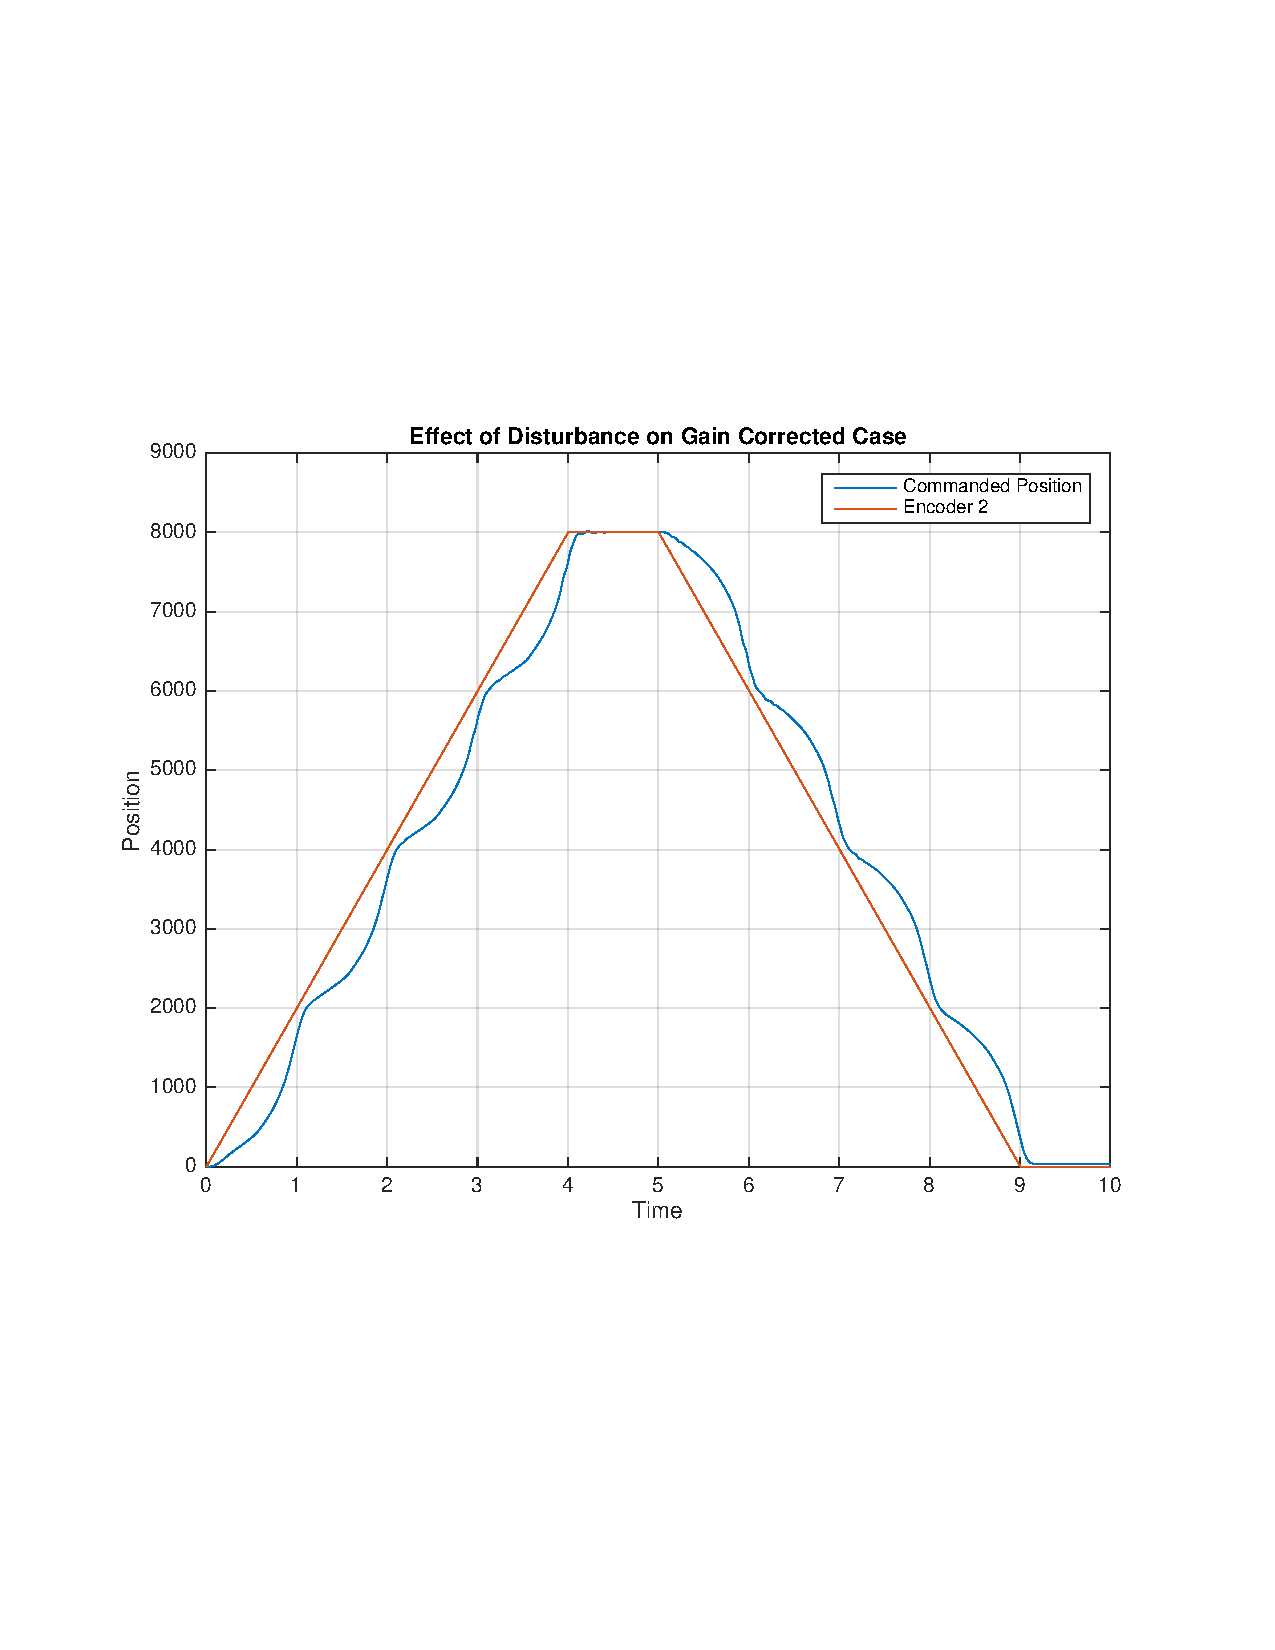
\includegraphics[width = \textwidth]{10_dist.pdf}
\end{figure}
\begin{figure}[H]
\centering
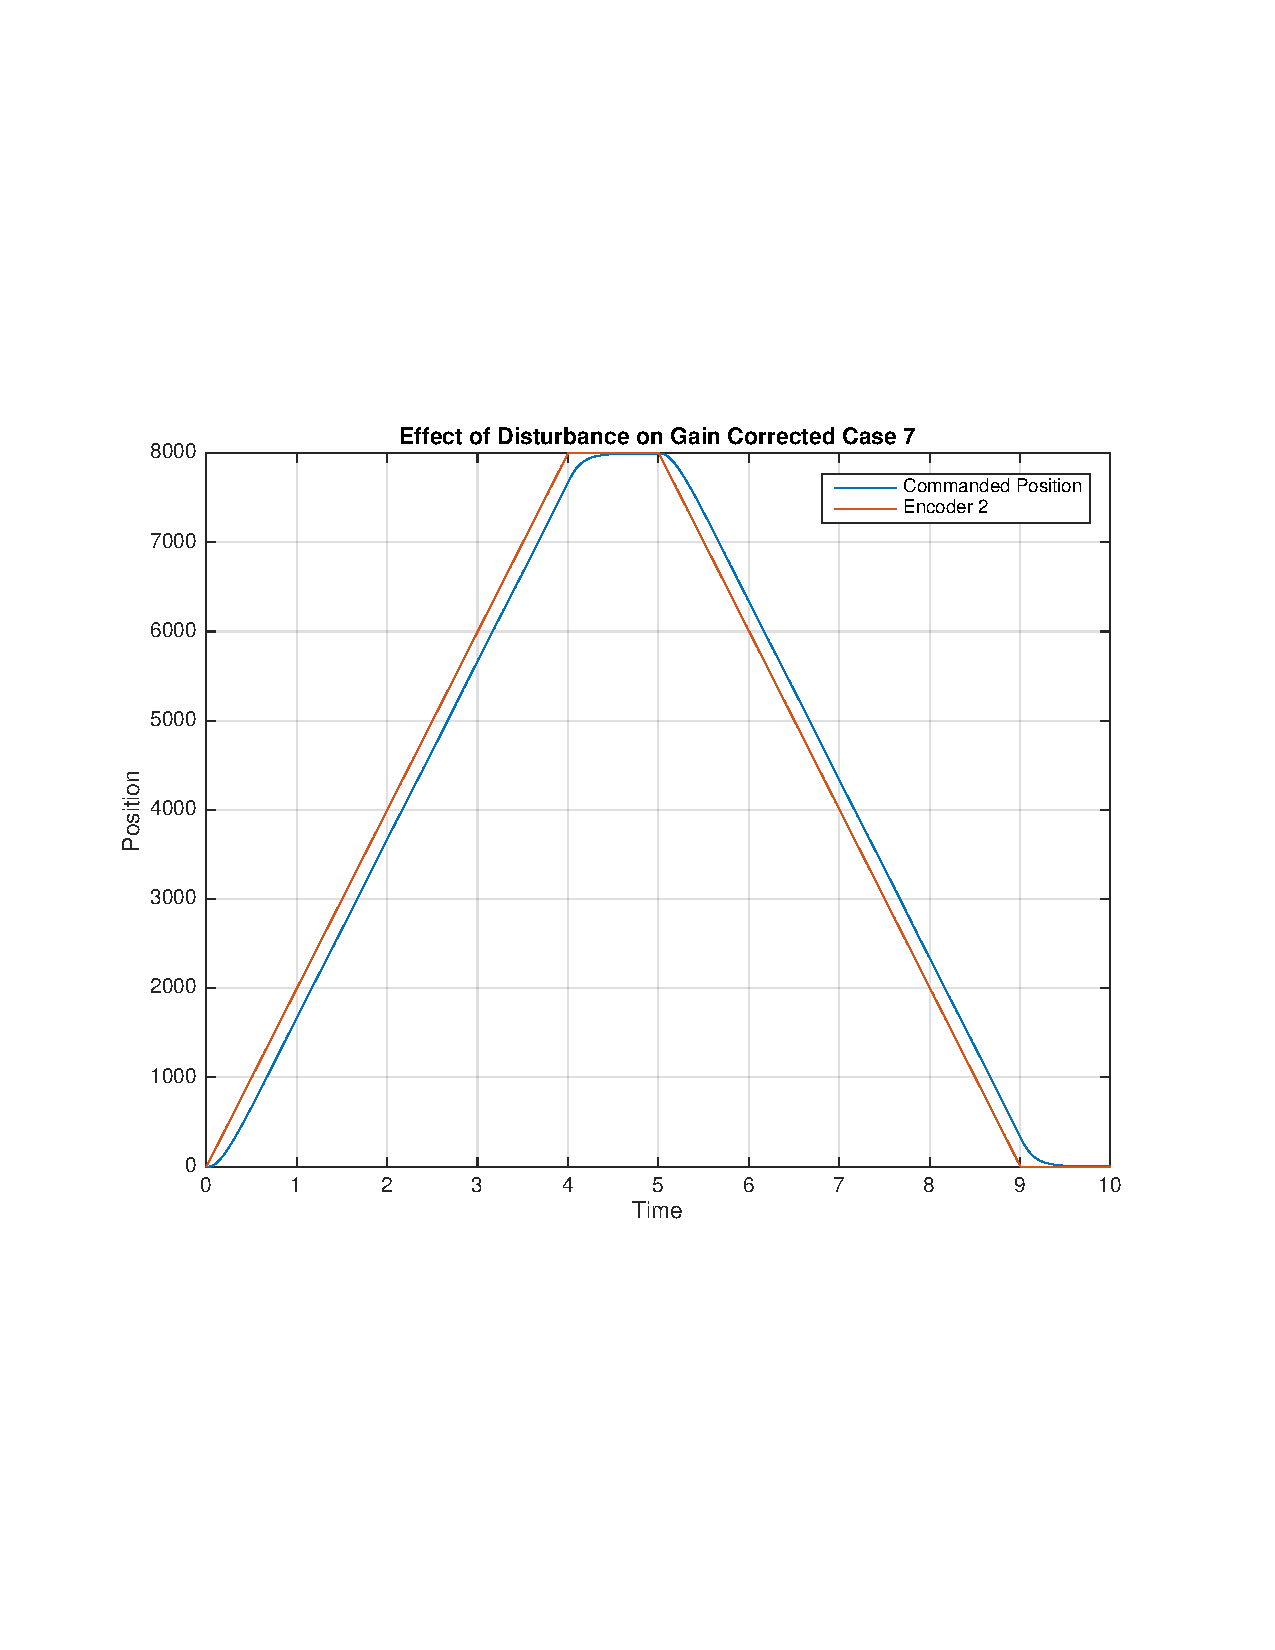
\includegraphics[width = \textwidth]{11.pdf}
\end{figure}
\section{Experiment- Control of Plant with Drive Flexibility}
In this section, we consider the implications of drive flexibility to plant control and implement several control schemes to mitigate its effect. The model of our plant belongs to a class having two degrees of freedom (DOF) corresponding to normal modes of oscillation (actually one oscillatory and one rigid body mode in our case) and hence is of fourth order. The block diagrams of the system for time and Laplace domain analyses are shown in Figure \ref{SIMO} which gives details of the location of $k_{hw}$ gain elements in the signal flow. The signals $\theta_1$ and $\theta_2$ are the respective angle measurements in encoder counts.
\begin{figure}{H}
\centering
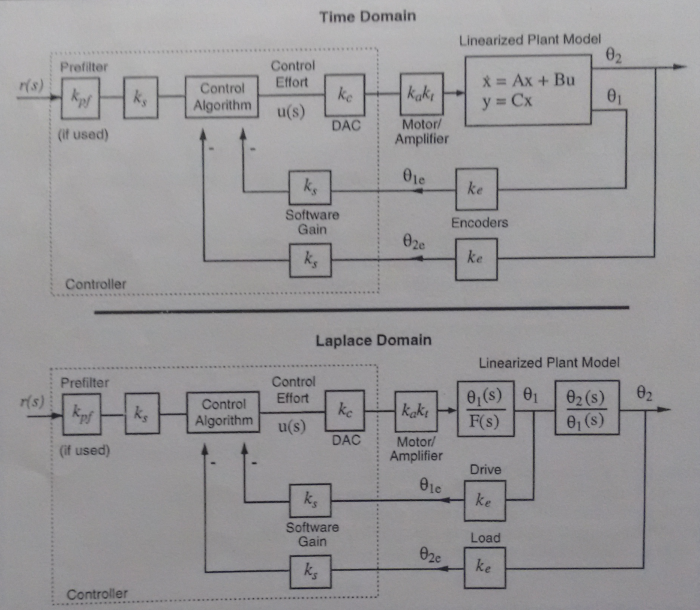
\includegraphics[width = \textwidth]{block_simo.png}
\caption{Block Diagram for 2 DOF Control(SIMO)}
\label{SIMO}
\end{figure}
\subsection{Collocated Control}
this experiment we consider PD control of the 2-disk system where the controlled output, $\theta_1$, is of the drive disk. Such a scheme is referred to as collocated since the sensor output is rigidly coupled to the actuator input.
\begin{enumerate}
\item Setup system as in test case 11.(figure \ref{Fig8})
\item Implement the following gains under PI with Velocity Feedback: $k_p = 0.1, k_d = 0.005,k_i = 0$ with Ts = 0.002652 s. Set-up data acquisition for encoders 1 and 2 and for commanded position and gather data every 5 servo cycles. Execute a 1000 count step response and plot the result for commanded position and encoder 1.
\item Now iteratively adjust the gains kp \& kd and plot results to obtain an improved response. Make your gain adjustments gradually (not more than 50$\%$ at a time) and note the effects of increasing or reducing each of them. Do not input $k_p = 1.5 or 0.005$ $k_d = 0.015$. Attempt to achieve performance goals of 100 ms rise time (0-90\% amplitude) and 10\% overshoot without excessive oscillation. Save your best step response plot. Manually displace the drive disk and note the relative stiffness of the servo system.
\item For your last iteration in Step 3, plot the step response of the load disk. (There is no need to rerun the step, simply re-setup the plot for ”encoder 2” \& ”commanded position” and plot data.)
\item Now using the existing values of $k_p \& k_d$ as starting points, iteratively change (lower) gains and plot $\theta_2$ results to provide a well-behaved step response with 10\% overshoot, without excessive oscillation, and as fast a rise time as possible. Save your final plot and record the corresponding gains. Manually displace the drive disk and note the relative stiffness.
\item Calculate the poles of the closed-loop transfer functions: $\theta_1$(s)/r(s) and $\theta_{12}$(s)/r(s) for your final controllers in Steps 3 \& 5 respectively
\item The torque from manually displacing the disk in Steps 3 \& 5 entered the system as the disturbance $T_d$.
\end{enumerate}
\subsubsection{Plots}
\begin{figure}[H]
\centering
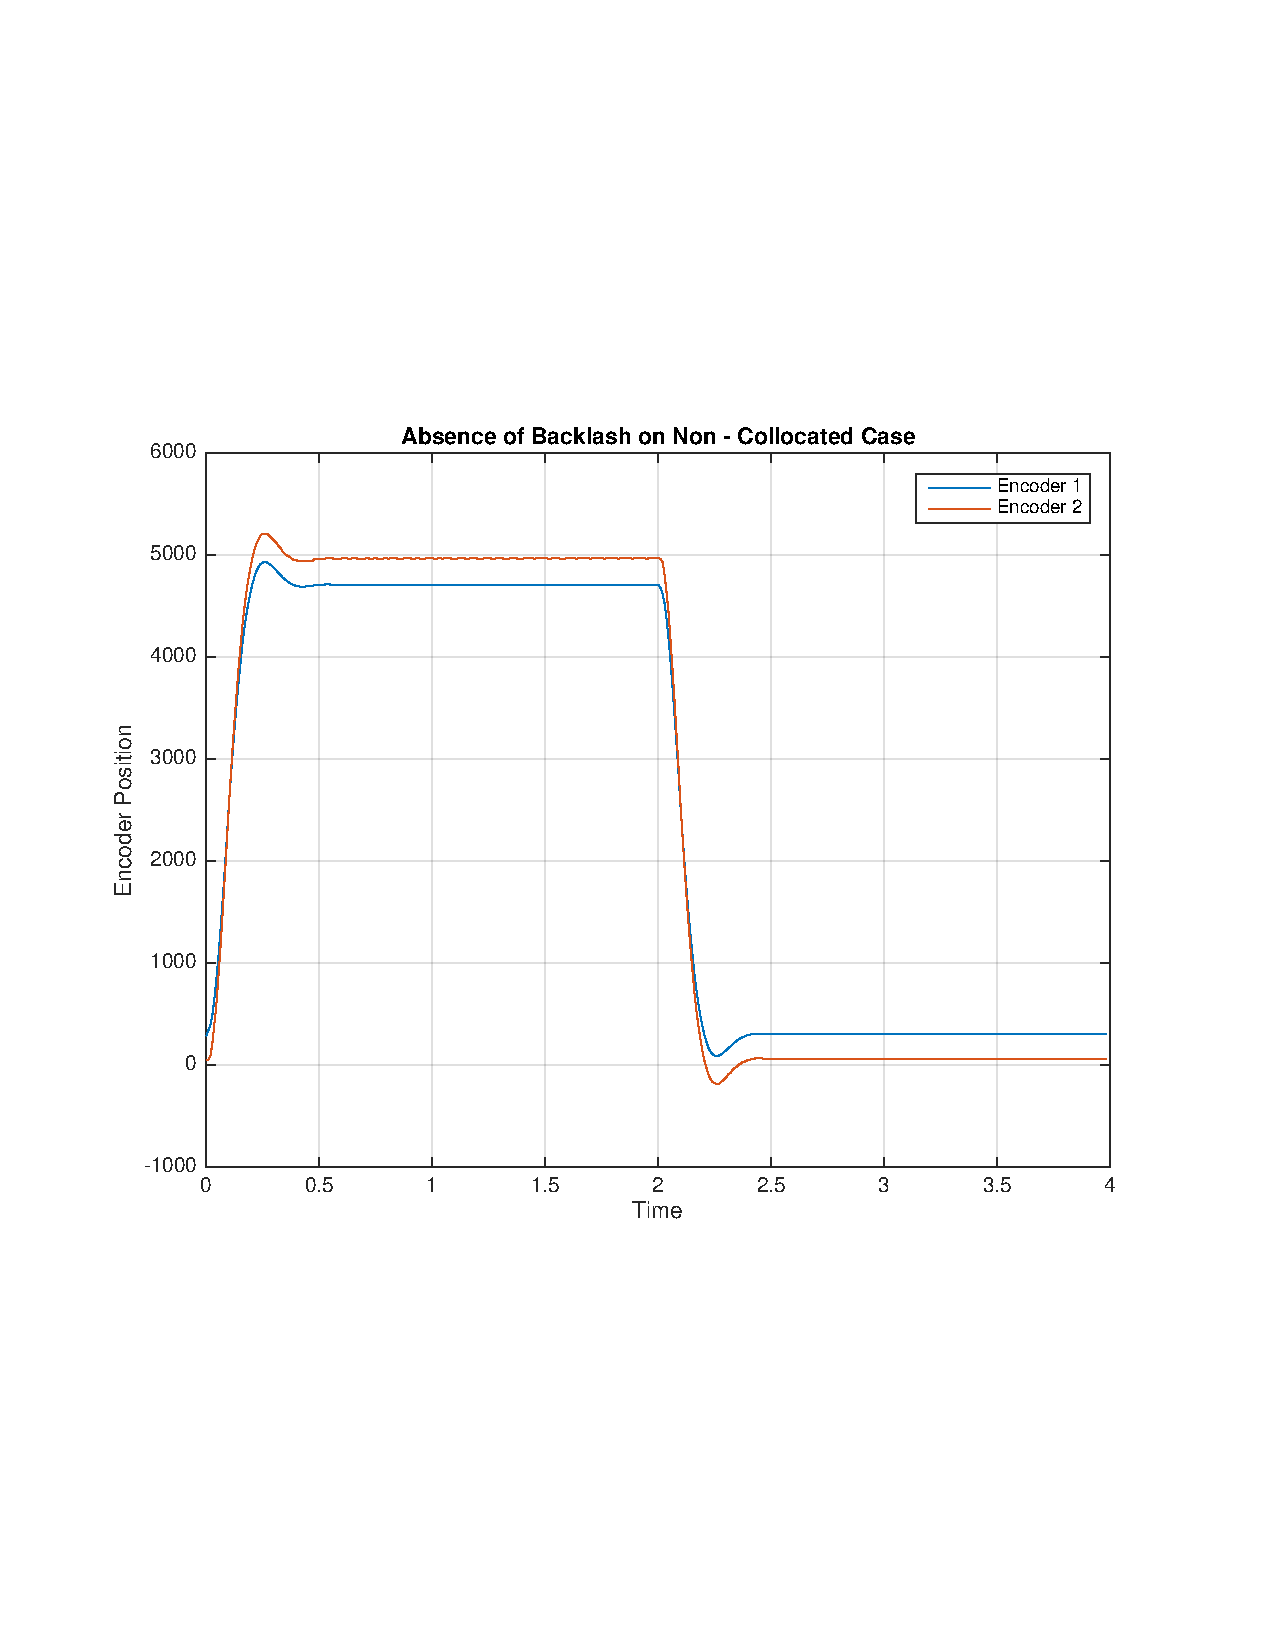
\includegraphics[width = \textwidth]{12.pdf}
\end{figure}
\begin{figure}[H]
\centering
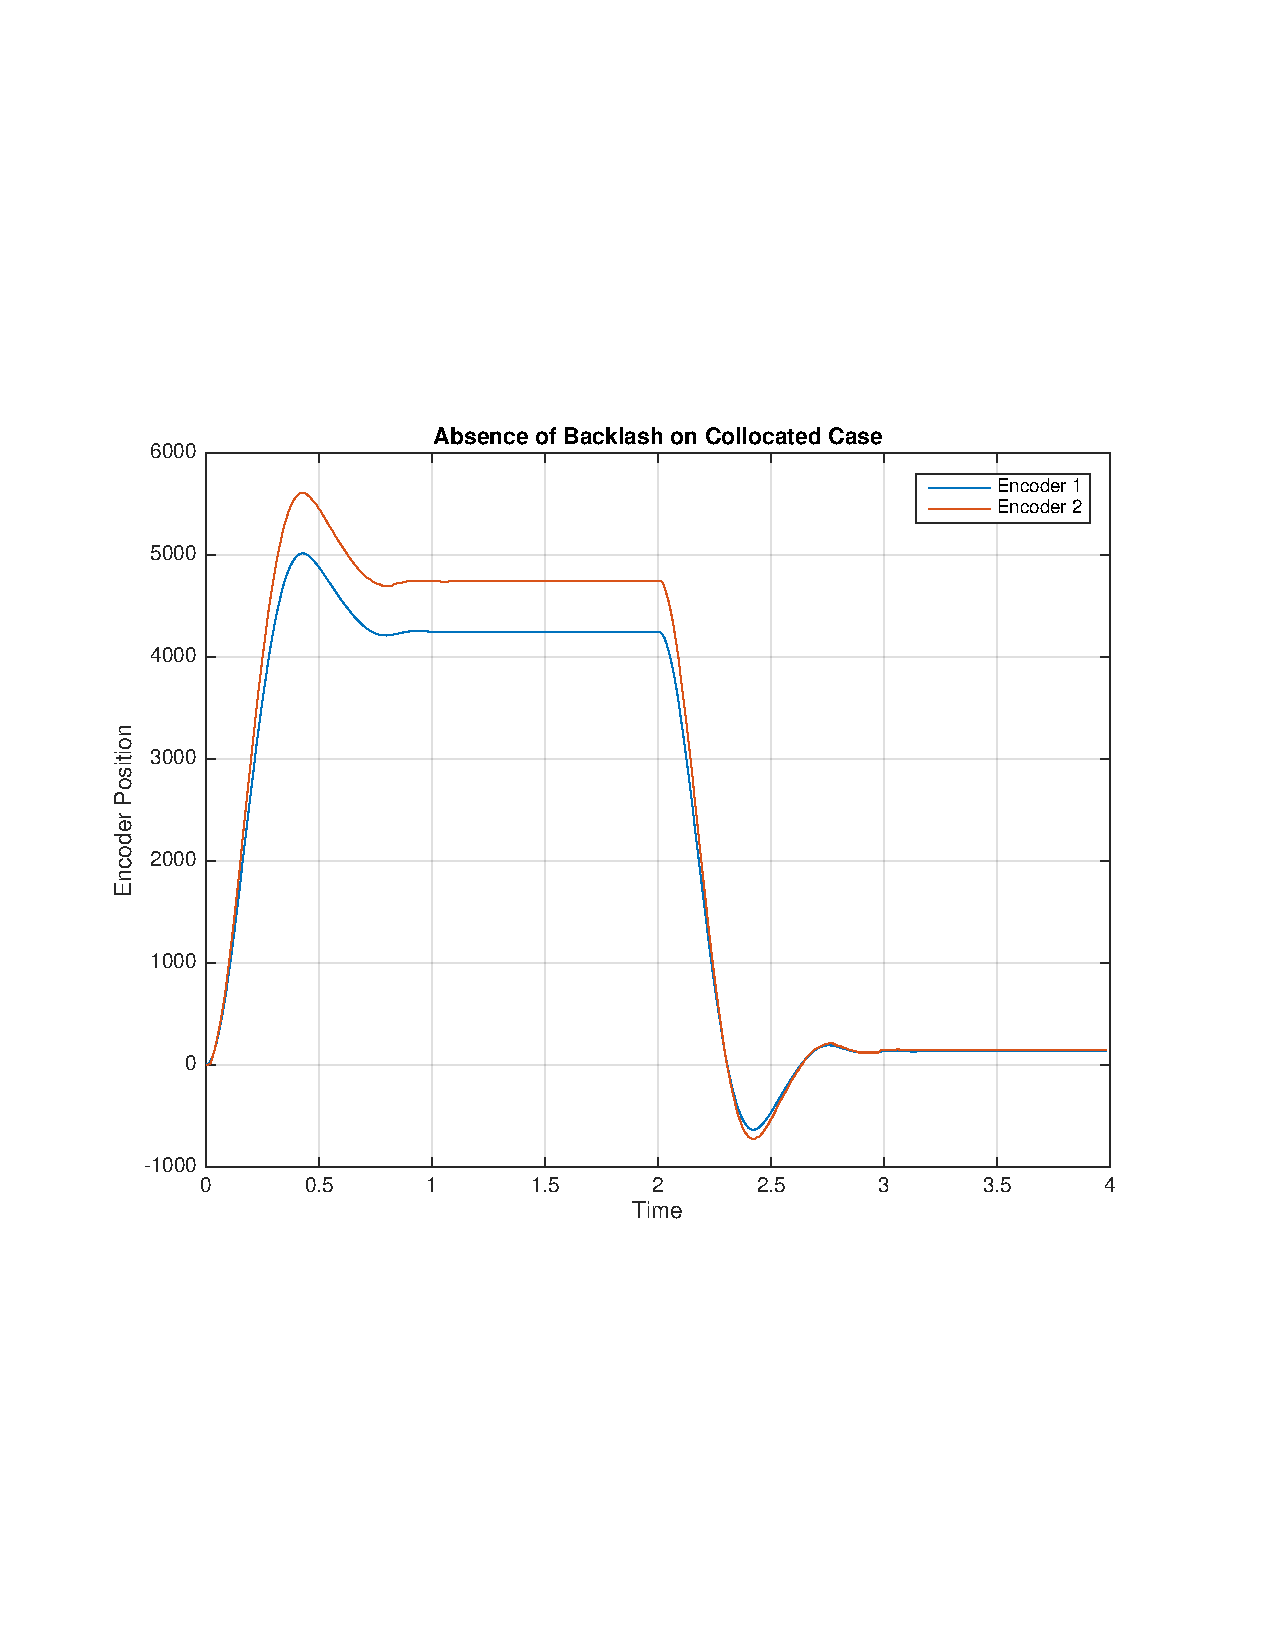
\includegraphics[width = \textwidth]{13.pdf}
\end{figure}
\begin{figure}[H]
\centering
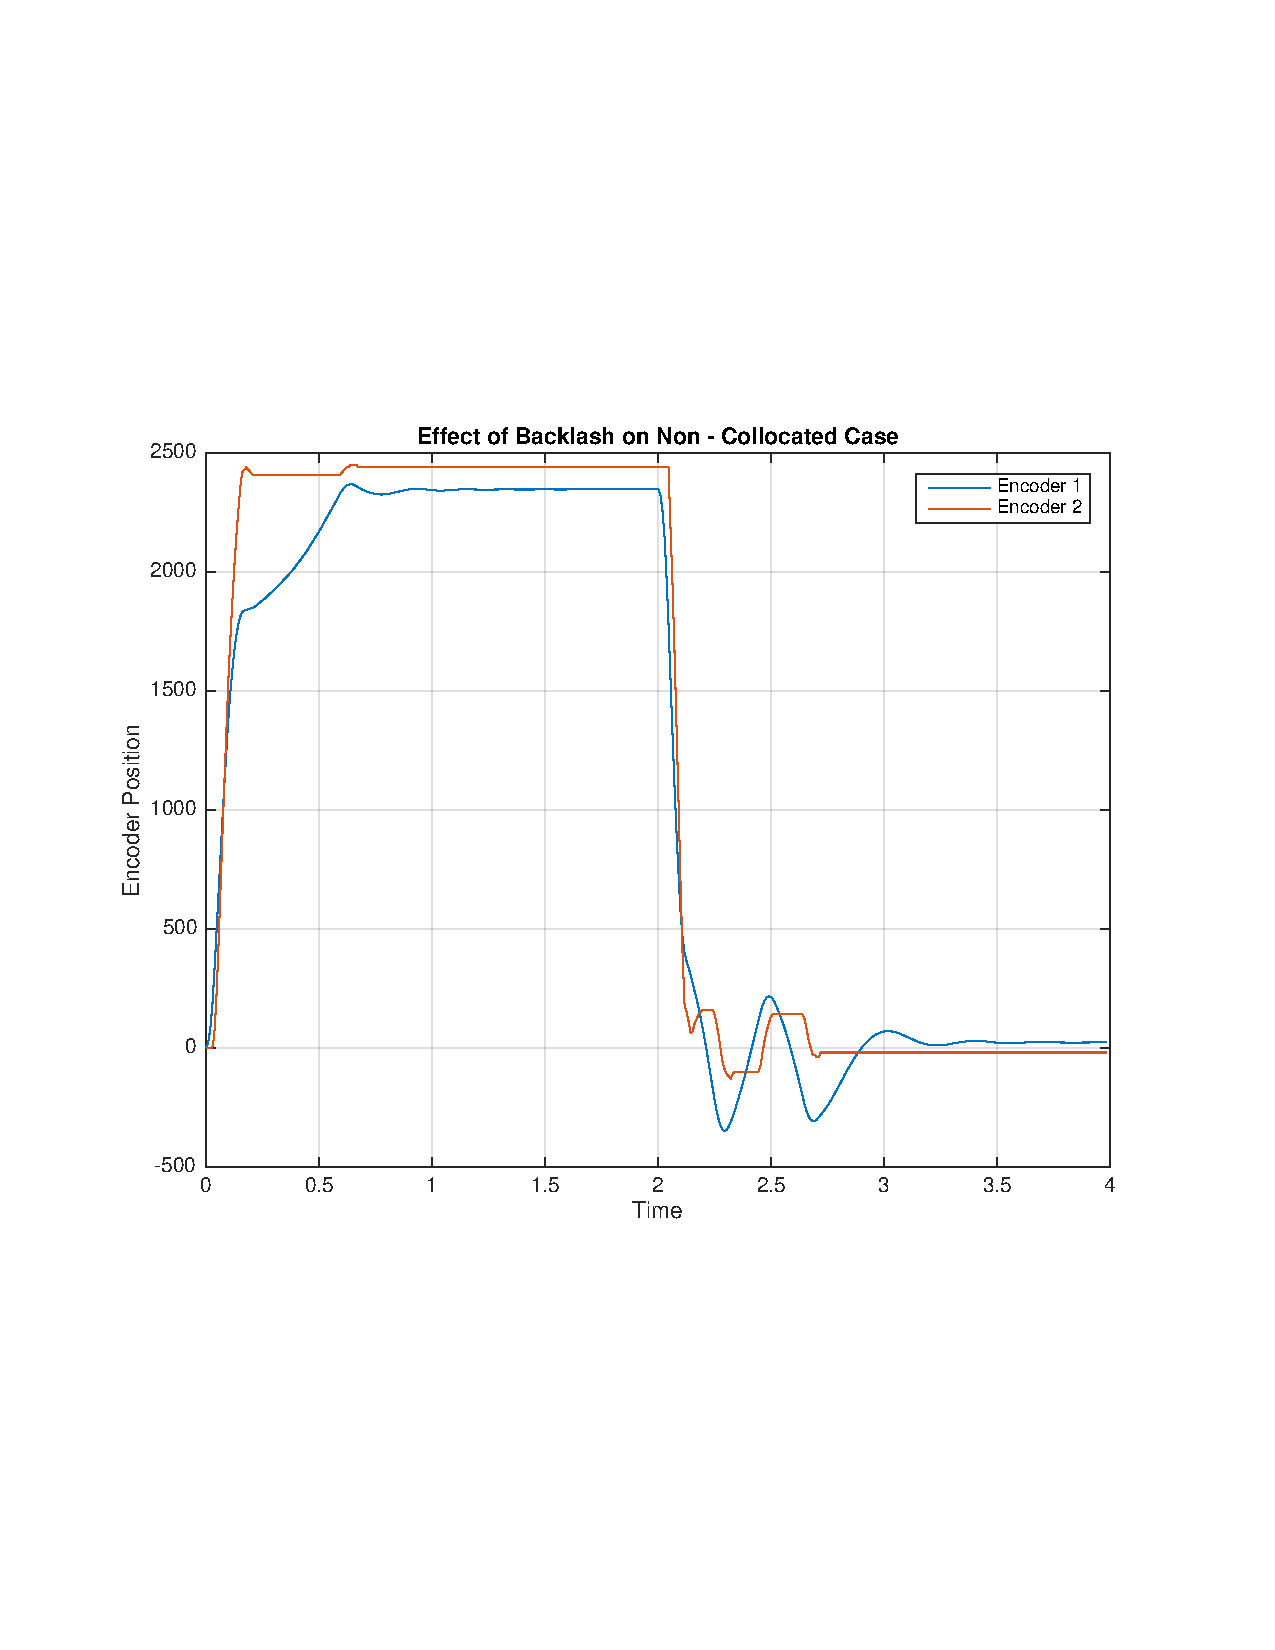
\includegraphics[width = \textwidth]{14.pdf}
\end{figure}
\begin{figure}[H]
\centering
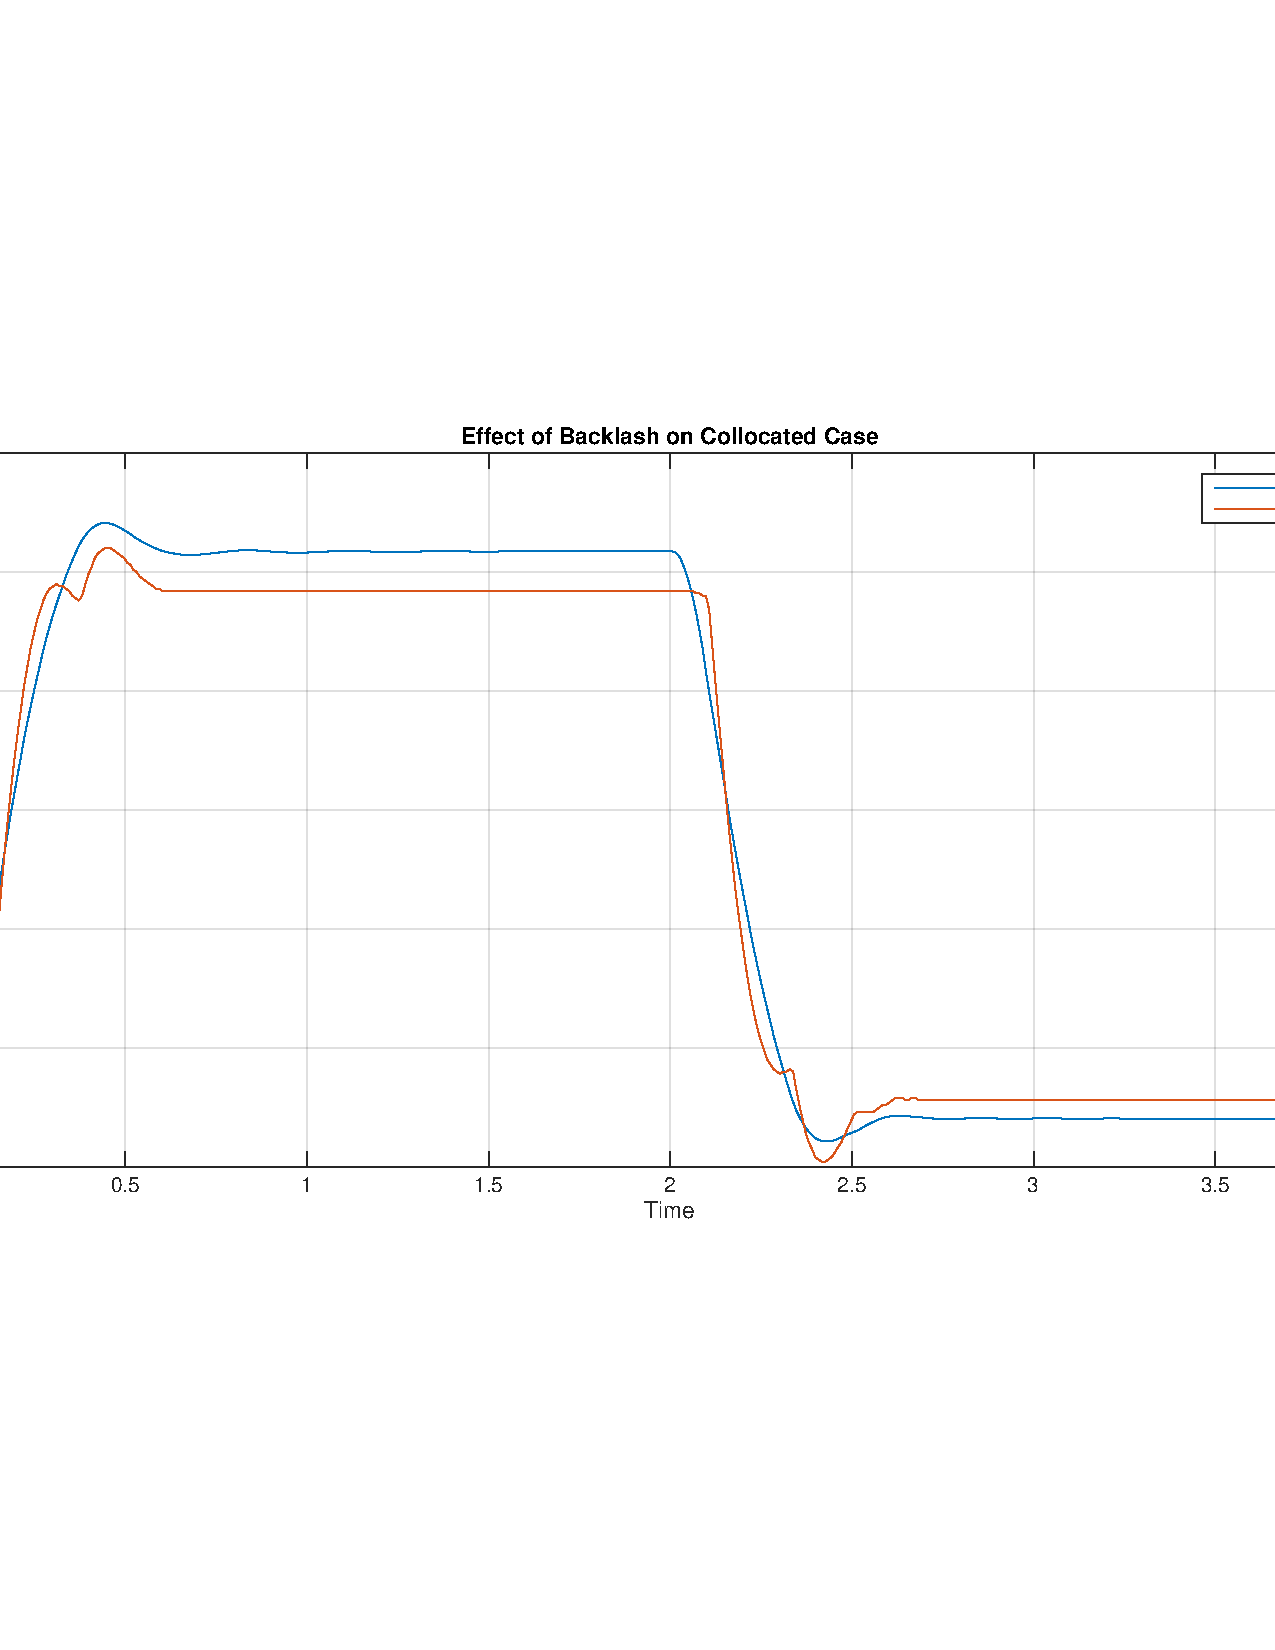
\includegraphics[width = \textwidth]{15.pdf}
\end{figure}
\end{document}